\title{Final Year Project}
\documentclass[12pt]{extarticle}
\usepackage{authblk}
\usepackage{times}
\usepackage{float}
\usepackage[utf8]{inputenc}
\usepackage{csquotes}
\usepackage{pdfpages}
\usepackage{setspace}
\usepackage{tabularx}
\usepackage{amsmath}
\usepackage{array} 
\usepackage{longtable}
\usepackage{listings}
\usepackage{array} % Add this in the preamble if not already there
\usepackage{makecell} % For better cell formatting
\usepackage[a4paper, margin=1in]{geometry}
\usepackage[backend=biber, sorting=none]{biblatex}

\addbibresource{references.bib}
\usepackage{listings}
\usepackage{xcolor}


\begin{document}
% We'll use the title page created separately and then later combine
% it with this document
\begin{titlepage}
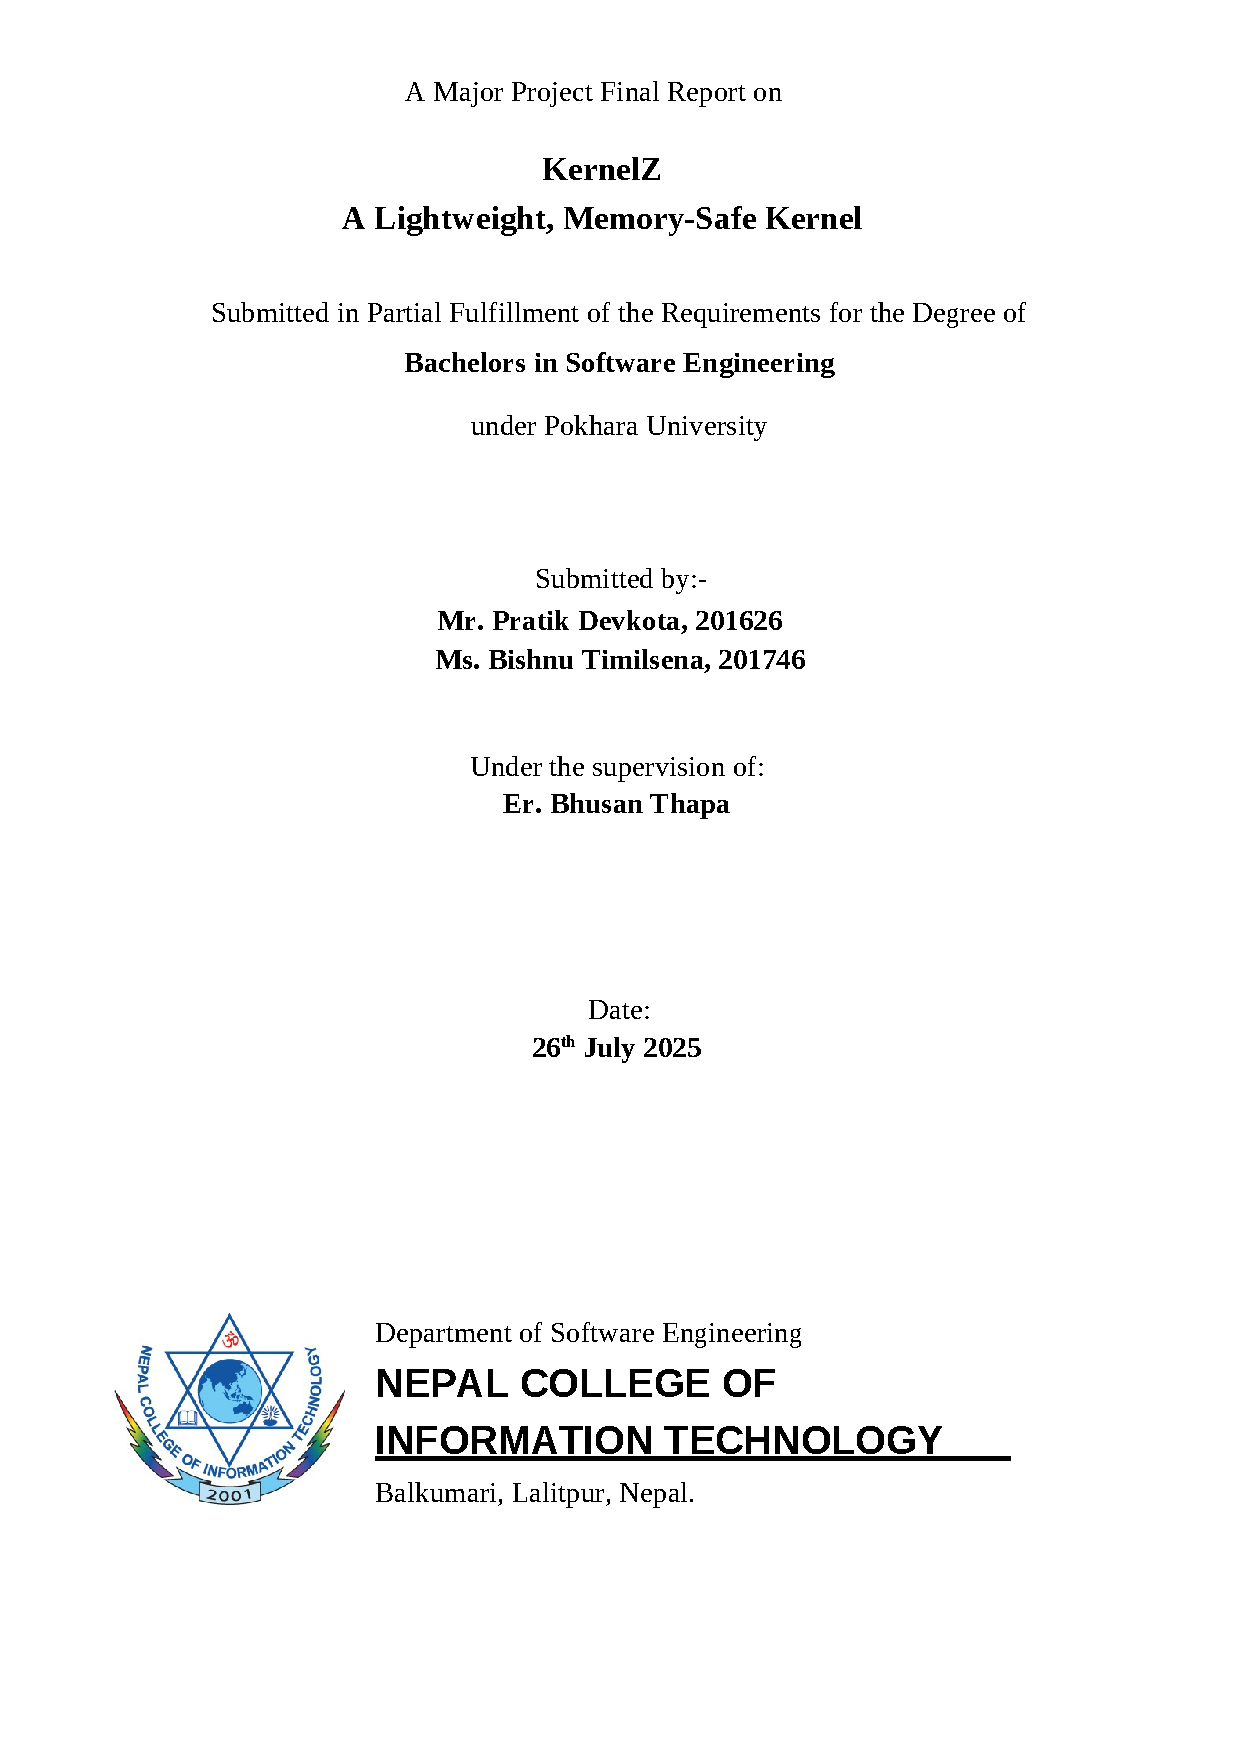
\includepdf{coverpage}
\end{titlepage}

\onehalfspacing % Set line spacing to 1.5

\pagenumbering{Roman}

\begin{center}
	\textbf{Acknowledgement}
\end{center}

\noindent We would like to express our sincere gratitude to everyone who contributed to the successful completion of the \textbf{KernelZ} project, a lightweight and memory-safe operating system kernel developed from scratch.

\noindent First, we extend our heartfelt thanks to our supervisor, Er. Bhusan Thapa, for his consistent guidance, insightful feedback, and technical mentorship throughout the project. His expertise in low-level systems programming played a vital role in shaping the architecture and direction of KernelZ.

\noindent We are equally grateful to the Nepal College of Information Technology for providing the academic platform, computing resources, and learning environment necessary to carry out such a challenging system-level project. The opportunity to work on real-world kernel development has been both enriching and transformative.

\noindent Our deepest appreciation also goes to all members of the development team for their dedication, collaboration, and perseverance. Each contributor brought unique strengths to the table,from memory model design and paging implementation to debugging and documentation, which were crucial to the overall success of the project.

\noindent In conclusion, the development of the KernelZ memory subsystem would not have been possible without the collective support and contributions of our supervisor, institution, and team members. We are truly grateful for this opportunity and look forward to building upon this foundation in future explorations of systems software and kernel engineering.

\medskip
\begin{flushleft}
KernelZ Development Team
\end{flushleft}
\pagebreak


\begin{center}
	\textbf{Abstract}
\end{center}
This project aims to develop \textbf{KernelZ}: a 64-bit operating system kernel
targeting the x86\_64 architecture, implemented using the Zig programming
language and the Limine bootloader. The kernel emphasizes modularity, memory
safety, and modern systems programming practices. It incorporates essential
low-level components including a physical and virtual memory manager, interrupt
handling through the Advanced Programmable Interrupt Controller (APIC), a
process scheduler, system call interface, and a minimal virtual file system.\\
\textbf{Keywords:} \textit{operating system}, \textit{kernel development}, \textit{Zig}, \textit{Limine bootloader}

\pagebreak

\tableofcontents

\pagebreak

\listoffigures

\pagebreak

\listoftables

\pagebreak

\renewcommand{\arraystretch}{1.5} % Row spacing for clarity
\section*{Abbreviations}

\begin{table}[H]
    \centering
    \begin{tabular}{|c|p{3.5cm}|p{10cm}|}
        \hline
        \textbf{S.N.} & \textbf{Acronym} & \textbf{Full Form} \\
        \hline
        1. & OS & Operating System \\
        \hline
        2. & API & Application Programming Interface \\
        \hline
        3. & IRQ & Interrupt Request \\
        \hline
        4. & IDT & Interrupt Descriptor Table \\
        \hline
        5. & GDT & Global Descriptor Table \\
        \hline
        6. & APIC & Advanced Programmable Interrupt Controller \\
        \hline
        7. & PIC & Programmable Interrupt Controller \\
        \hline
        8. & VFS & Virtual File System \\
        \hline
        9. & PIT & Programmable Interval Timer \\
        \hline
        10. & HPET & High Precision Event Timer \\
        \hline
        11. & QEMU & Quick Emulator \\
        \hline
        12. & GDB & GNU Debugger \\
        \hline
        13. & VMM & Virtual Memory Manager \\
        \hline
        14. & SMP & Symmetric Multi-Processing \\
        \hline
        15. & KASLR & Kernel Address Space Layout Randomization \\
        \hline
        16. & POSIX & Portable Operating System Interface \\
        \hline
        17. & MADT & Multiple APIC Description Table \\
        \hline
        18. & ELF & Executable and Linkable Format \\
        \hline
        19. & CR3 & Control Register 3 \\
        \hline
    \end{tabular}
\end{table}

\pagebreak

\setcounter{page}{1}

\pagenumbering{arabic}

\section{Introduction}
\subsection{Introduction}
Operating systems are crucial for modern computing, yet many educational kernels remain outdated, insecure, or overly complex. This project introduces KernelZ, a clean 64-bit educational operating system written in Zig, designed to bridge the gap between modern architecture, memory safety, and learnability.

\subsection{Problem Statement}
Operating systems are fundamental to the functioning of modern computing
systems, serving as the critical layer that manages hardware resources and
enables user-level applications to function. However, most of the educational
kernels we looked at were dominated by legacy architectures, outdated boot
methods, and unsafe programming practices rooted in languages like C. Moreover,
many existing kernels available for learning are either 32-bit, rely on legacy
features like the 8259 PIC instead of the modern APIC architecture, or lack
advanced components such as multitasking, userspace, and virtual memory.

While modern kernels written in safer languages like Rust exist, they are often
too large, complex, and not beginner-friendly, making them difficult to study or
contribute to. In contrast, Zig - a relatively new systems programming language
- offers a cleaner alternative with deterministic memory management and minimal
hidden control flow, making it ideal for educational purposes and safer
low-level systems development.

This project aims to address this gap by building a 64-bit educational operating
system kernel from scratch using Zig and the Limine bootloader. The project not
only helps the developers deepen their understanding of computer science
concepts - including memory management, hardware abstraction, interrupt
handling, system calls, and scheduling - but also contributes an approachable,
modern reference implementation to the open-source community.

\pagebreak

\subsection{Project Objectives}
    The primary objectives of the project are as follows:
    \begin{enumerate}
    \item To develop a operating system kernel targeting the \textit{x86\_64} architecture.
    \item To contribute a well-documented, beginner-friendly open-source kernel
    for the students interested in systems programming.
    \item To experiment with OS development concepts, kernel design and modern system architectures.
    \end{enumerate}

\pagebreak

\subsection{Significance of the Study}

This study is significant for several reasons. First, it provides a practical
and educational exploration of operating system internals using a modern
toolchain. Unlike many existing kernels that are built using outdated methods or
unsafe practices, this project embraces modern architectural features available
with the x86\_64 architecture thus offering a contemporary and relevant learning
experience.

Second, it contributes to the open-source ecosystem by offering a minimal,
well-structured, and thoroughly documented kernel that balances educational
clarity with real-world relevance. This is especially beneficial for students,
and self-learners who are interested in systems programming but often find
existing resources either too outdated or too complex to follow.

Finally, by adopting safer systems programming principles and building on a
modern stack, the project serves as a stepping stone for future research and
development in both academic contexts. It demonstrates that it is possible to
build performant and low-level software without compromising on safety or
maintainability - qualities that are increasingly important in contemporary
software engineering.

\pagebreak

\subsection{Scope and Limitations}

\subsubsection*{Scope}
This project focuses on the development of a 64-bit monolithic kernel for the
\textit{x86\_64} architecture. The kernel includes fundamental components
such as:

\begin{itemize}
    \item Memory management including paging mechanisms and virtual memory allocators
    \item Interrupt handling using the APIC and programmable timers
    \item Basic input/output support (e.g., keyboard, screen via video mode)
    \item Basic task scheduling
\end{itemize}

The project is educational in nature, aiming for simplicity, and clarity rather
than completeness or performance. It serves as both a learning tool for the
developers and a reference implementation for other learners.

\subsubsection*{Limitations}
Given time and resource constraints, the following features are beyond the
current scope of the project:

\begin{itemize}
    \item Support for multiple hardware architectures (e.g., ARM, RISC-V)
    \item Advanced features like SMP (Symmetric Multi-Processing), advanced filesystems, networking, and security enforcement (e.g., KASLR)
    \item Full POSIX compliance or support for running complex userspace
    programs
    \item Graphical display output or drivers beyond basic text
    \item Persistent storage drivers or disk-based filesystems
\end{itemize}

The kernel is not intended for production use but rather for educational
exploration of low-level system design. Future work may extend the project to
include more robust features and broader hardware support.

\pagebreak

\section{Literature Review}

Operating system kernels interface directly with hardware and manage critical
resources such as memory, processor scheduling, and input/output devices.
Ensuring memory safety within kernel code is essential due to the high risks
associated with vulnerabilities like buffer overflows, use-after-free, integer
overflows, and dangling pointers. This literature review covers the key concepts
relevant to developing a memory-safe kernel using Zig, Limine, and QEMU.

\subsection{Historical Evolution of Operating System Kernels}

The concept of an operating system kernel evolved alongside the increasing complexity of computing hardware. Early computers in the 1940s and 1950s operated without operating systems, relying on manual job execution via punched cards or switches, resulting in inefficient CPU utilization~\cite{tanenbaum2015}. This led to the development of batch processing systems like IBM's GM-NAA I/O, which introduced job automation and primitive scheduling~\cite{silberschatz2018}.
\vspace{1em}

The 1960s introduced time-sharing systems such as MIT's CTSS and IBM's OS/360, which formalized kernel responsibilities like process isolation and memory protection~\cite{ceruzzi2003}. By the 1970s, UNIX brought the monolithic kernel model into prominence, integrating all core OS functions into a single address space for performance and portability~\cite{ritchie1974}.
\vspace{1em}

In the 1980s, microkernels such as Mach and MINIX emerged, moving non-essential services to user space to improve modularity, although at a performance cost. This eventually led to hybrid kernels in the 1990s, such as Windows NT and Apple's XNU, which combined monolithic speed with microkernal structure~\cite{russinovich2017}.
\vspace{1em}

Today's kernels continue to evolve, incorporating modularity, real-time support, and enhanced security. Modern innovations include exokernels and unikernels for cloud-native workloads, along with secure extensions like SELinux and lightweight microVM kernels like Firecracker~\cite{kaashoek1997}.

\subsection{Freestanding Kernel Development}

A freestanding kernel operates independently of any host operating system or
standard runtime libraries, requiring explicit management of the memory layout,
stack initialization, and entry point execution. Typically, such kernels
necessitate carefully structured linker scripts and customized cross-compilation
toolchains (e.g., targeting the \textit{x86\_64-elf} binary format) to ensure
isolation from host system dependencies~\cite{osdev2025}.

\subsection{Bootloader Integration with Limine}

Limine is an advanced, modular bootloader with its own boot protocol, providing
essential features such as structured memory maps, framebuffer, and kernel image
loading capabilities~\cite{limine_bootloader}. It enables higher-half kernel loading, simplifying memory
addressing and comes built-in with the necessary setups (like PAE, Page tables,
GDT).

\subsection{Memory Safety in Kernel Programming}

Traditional languages like C/C++ dominate kernel programming but introduce
significant memory safety risks due to manual memory management. Modern
languages such as Rust address these risks through enforced memory management
rules (borrow-checker, ownership)~\cite{rustsafety}, though at times these
constraints complicate kernel-level programming due to the frequent necessity
for unsafe code blocks.

\subsection{Zig as a Modern Systems Programming Language}

Zig represents a modern approach to systems programming by explicitly managing
memory without hidden behaviors, providing clearer error handling, and allowing
precise control of the compilation process~\cite{ziglang}. Zig's capability to
be able to use some of the standard library features even on freestanding kernel
development, offering direct control over low-level system interactions without
the overhead or complexity often associated with Rust~\cite{radisic_zig_vs_rust}.

\subsection{Debugging and Emulation with QEMU}

QEMU~\cite{qemu_docs} serves as an emulator and debugging platform for kernel
development, providing an isolated environment for early kernel testing.
Integrated with tools like GDB~\cite{gdb_docs}, QEMU facilitates real-time debugging, step-wise
execution tracing, and memory analysis.
\newpage

\section{Methodology}

This section includes the methodology that is being followed during the development of the operating system project.

\subsection{Kernel Architecture}

KernelZ adopts a \textbf{monolithic kernel architecture}, in which all core
operating system services including memory management, interrupt handling,
process scheduling, device drivers, and system call handling operate within the
same privileged address space (ring 0). This unified structure enables direct
function calls across subsystems, reducing the overhead associated with
inter-process communication and context switching.

\begin{figure}[h]
    \centering
    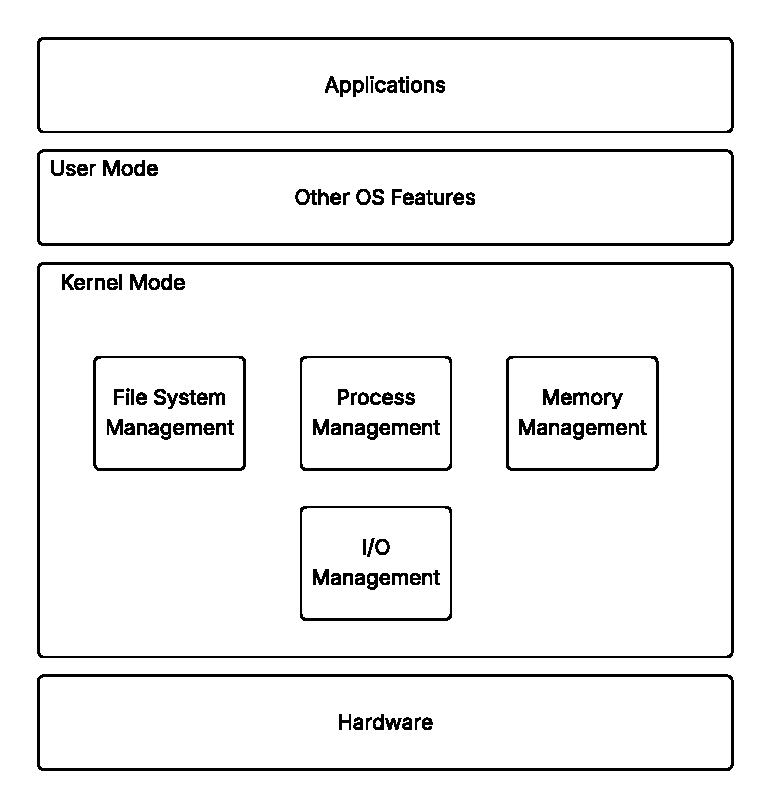
\includegraphics[width=0.8\textwidth]{figures/Monolithic architecture.pdf}
    \caption{Monolithic Architecture}
    \label{fig:enter-label}
\end{figure}

The monolithic model was selected due to its simplicity, performance efficiency,
and suitability for low-level educational kernel development. By maintaining a
shared execution context, this architecture facilitates rapid prototyping,
easier debugging, and tighter integration of kernel components, all of which are
critical during early-stage systems programming.

Alternative models, such as microkernels, offer advantages in modularity and
fault isolation by running most services in user space. However, they also
introduce considerable complexity in terms of IPC mechanisms, context
management, and driver separation. For this project, which emphasizes clarity,
minimalism, and foundational understanding, a monolithic architecture was deemed
more practical and aligned with the project's goals.

In summary, KernelZ leverages the performance and integration benefits of a
monolithic kernel to provide a clean, maintainable, and educationally rich
platform for exploring modern operating system concepts.
\pagebreak

\subsection{Software Development Life Cycle}
We follow an Iterative and Incremental Software Development Model, organizing
our 70-day timeline into four structured iterations. This allows for continuous
integration, early feedback, and the delivery of working subsystems at the end
of each iteration.

\begin{figure}[h]
    \centering
    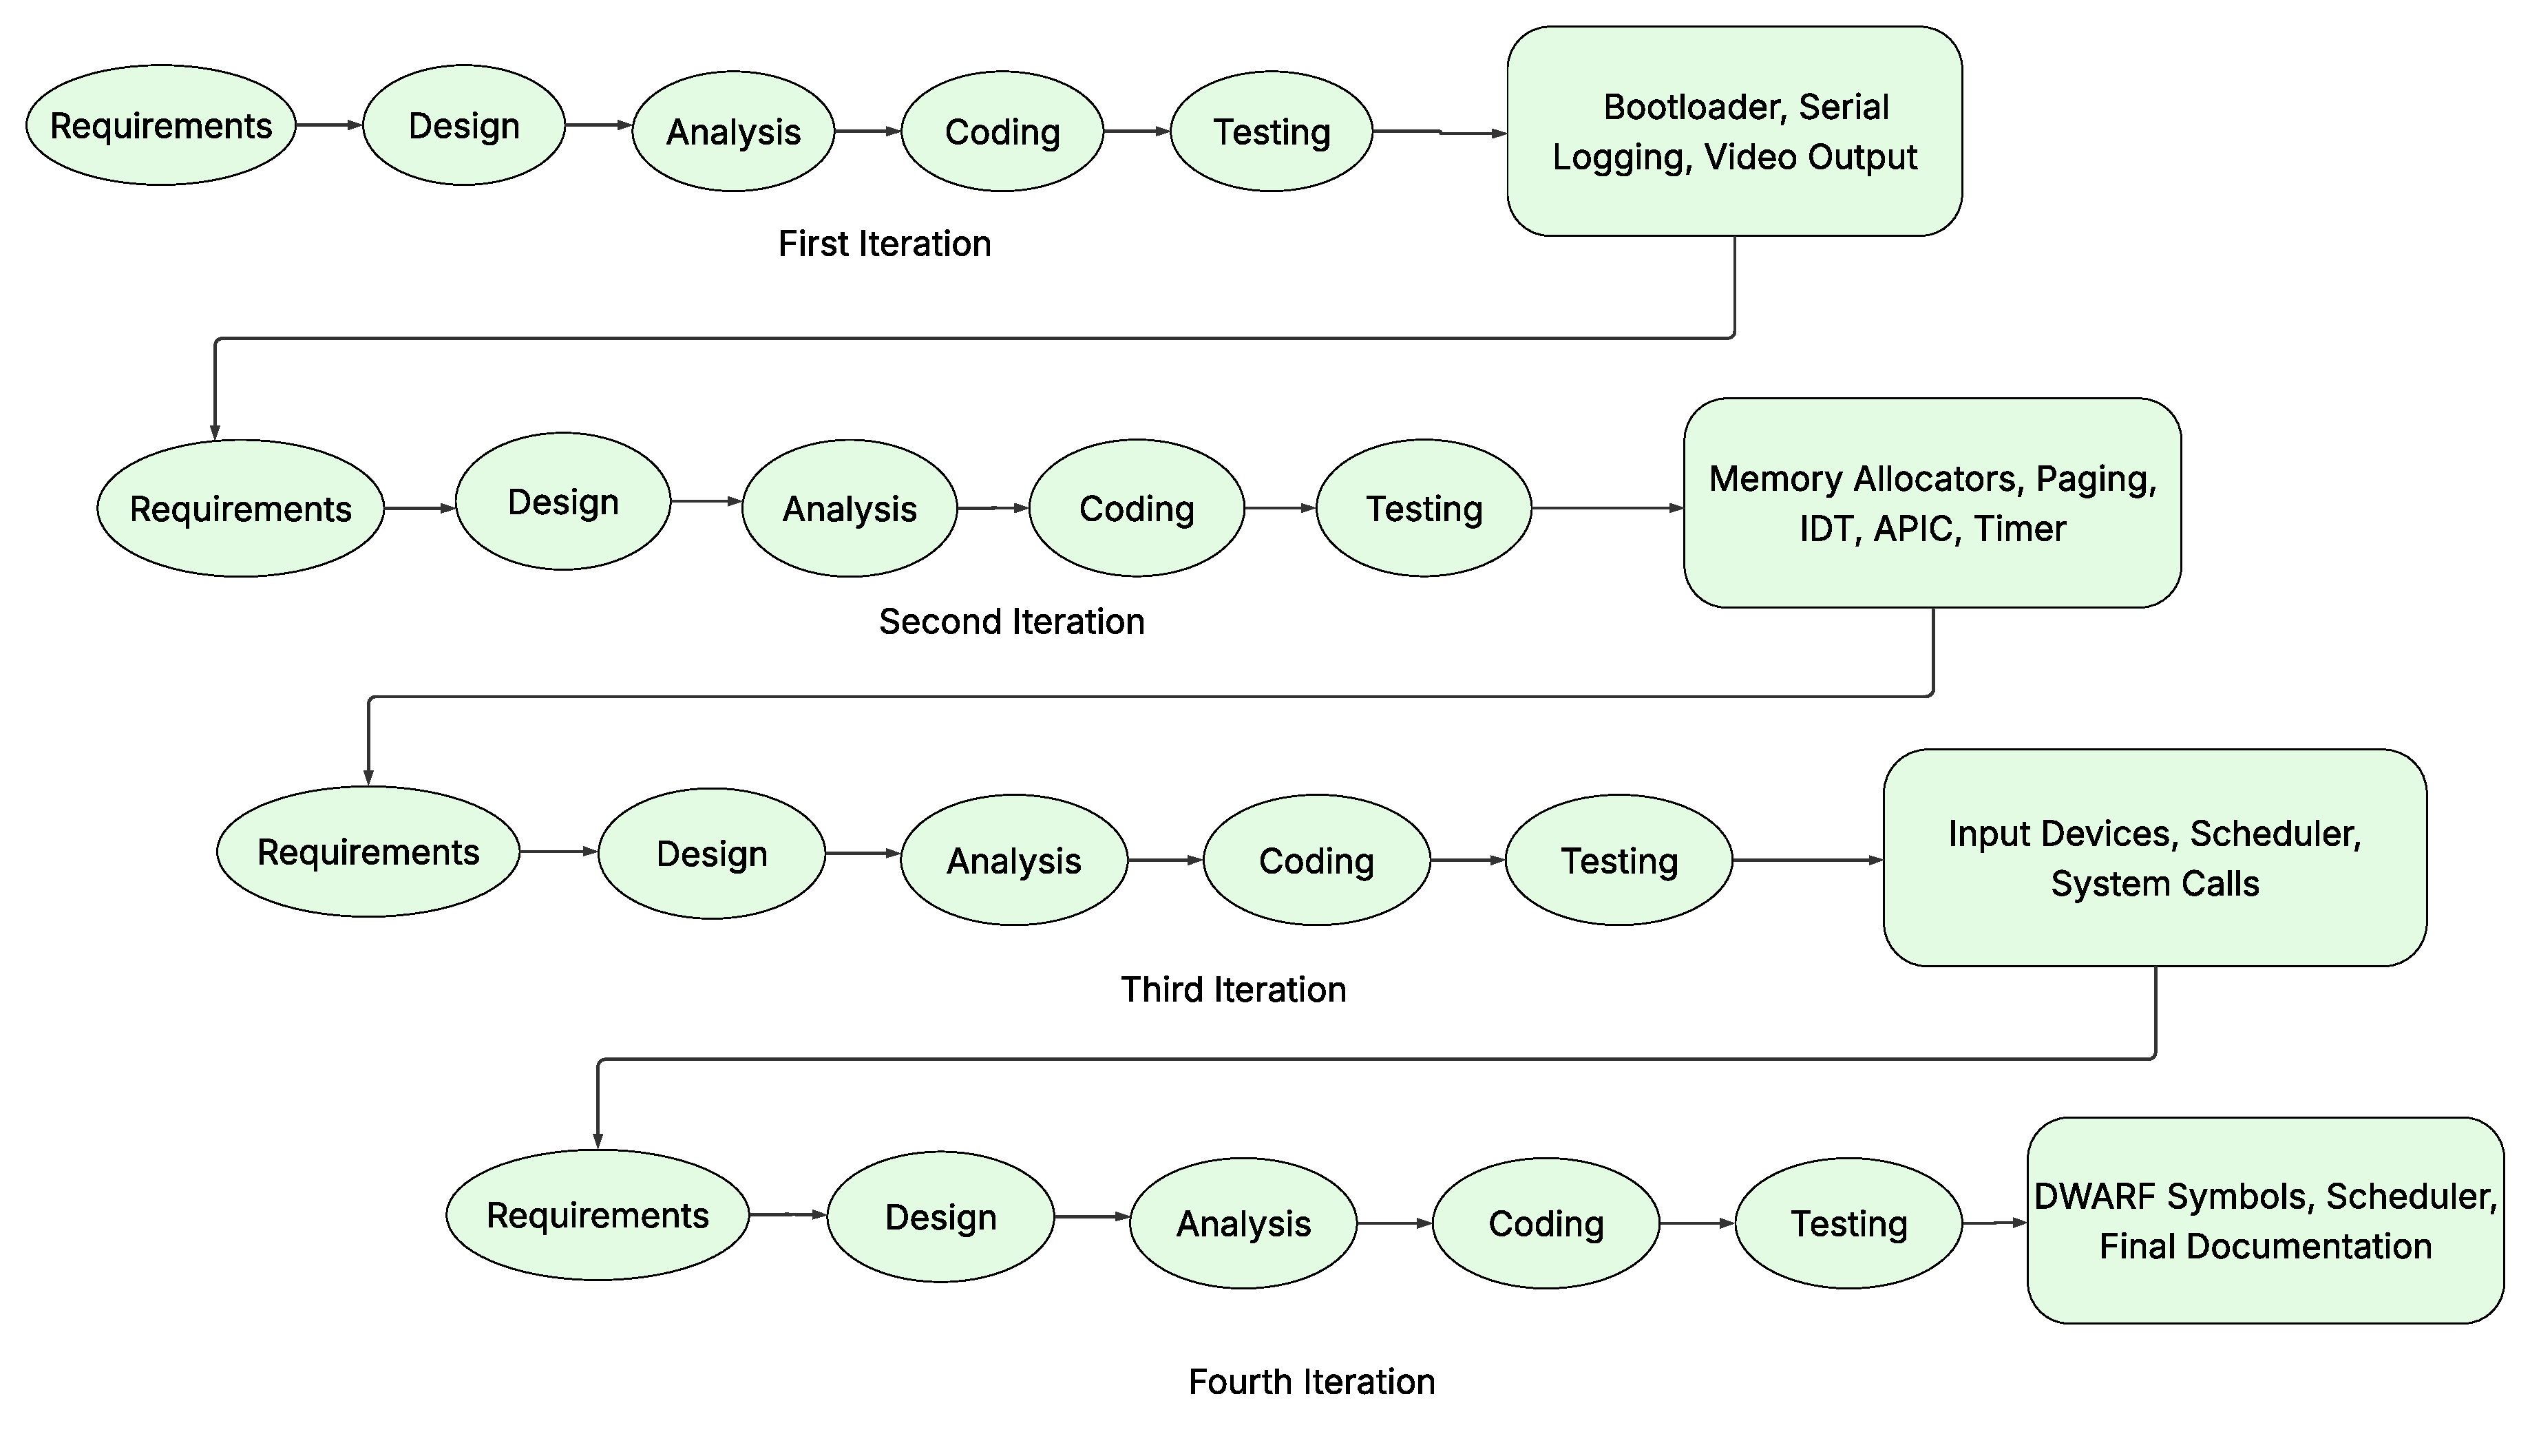
\includegraphics[width=\textwidth]{figures/Iterative and Incremental model.pdf}
    \caption{Incremental Model}
    \label{fig:Increment Model}
\end{figure}
\subsubsection*{Iteration 1: Bootstrapping and Framebuffer Output}

The first iteration focuses on establishing the initial boot sequence and
enabling visual output through framebuffer graphics. The Limine bootloader is
configured to load the kernel, and framebuffer-based terminal rendering is
implemented to provide immediate visual feedback during early-stage kernel
development. A development infrastructure, including build scripts (Makefiles,
Zig Build System), basic debugging utilities (gdb), and logging mechanisms via
serial ports, are established.

\subsubsection*{Iteration 2: Memory Management, Keyboard, Timer, and Interrupts}

In the second iteration, critical architectural elements necessary for hardware
interaction and efficient memory allocation are introduced. The Global
Descriptor Table (GDT) is configured to manage memory segments, and the
Interrupt Descriptor Table (IDT) is set up for handling interrupts and
exceptions. Advanced interrupt handling capabilities are developed through the
IO APIC, configured dynamically using the ACPI Multiple APIC Description Table
(MADT) for precise interrupt routing. A physical memory frame allocator and a
virtual memory system leveraging paging mechanisms are implemented, enabling
dynamic memory management and protection. Additionally, interrupt-driven drivers
for the keyboard and programmable timer devices (PIT or HPET) are created to
provide responsive and interactive user experiences.

\subsubsection*{Iteration 3: System Calls, Scheduler, and IRQs via APIC}

The third iteration addresses the implementation of multitasking and user-kernel communication. A cooperative scheduler is designed and integrated, utilizing timer interrupts to facilitate task switching and basic multitasking capabilities. System call support is established, either through the syscall/sysenter mechanism or via designated software interrupt vectors, enabling structured interactions between user applications and kernel-level services. The IRQ handling mechanism is expanded and thoroughly tested with APIC-based interrupts, ensuring stable, efficient, and scalable communication between software and hardware components.

\subsubsection*{Iteration 4: File System, Integration, and Final Documentation}

The final iteration emphasizes storage management, comprehensive system integration, and thorough documentation. An in-memory virtual file system (VFS) layer is developed, supporting essential file operations including reading, writing, and directory management. System components such as memory management, interrupt handling, device drivers, multitasking scheduler, and system call interfaces—are rigorously integrated, tested, and debugged, culminating in a stable and functional kernel environment. This iteration also includes the creation of detailed final documentation, encompassing system architecture descriptions, design decisions, usage guides, and comprehensive technical references to support future development and maintenance activities.
\pagebreak


\subsection{Proposed Tools and Technologies}

Table~\ref{tab:techs} displays the tools and technologies intended for
employment in this project.

\renewcommand{\arraystretch}{1.5} % Consistent vertical spacing
\begin{table}[H]
    \centering
    \begin{tabular}{|c|p{4cm}|p{9cm}|}
        \hline
        \textbf{S.N.} & \textbf{Tool} & \textbf{Purpose} \\
        \hline
        1. & Zig & Kernel development \\
        \hline
        2. & Make & Build system automation \\
        \hline
        3. & Limine & Bootloader for launching the kernel \\
        \hline
        4. & QEMU & Hardware emulation and virtual machine testing \\
        \hline
        5. & Git & Version control and team collaboration \\
        \hline
        6. & \LaTeX{} & Project documentation formatting \\
        \hline
    \end{tabular}
    \caption{Proposed Tools and Technologies}
    \label{tab:techs}
\end{table}

\subsubsection*{Justification for Selection}

\paragraph{Zig:}
Zig is a modern low-level programming language that offers manual memory control
and highly predictable behavior. It supports freestanding kernel development
with minimal runtime dependencies, making it particularly suited for systems
programming. Zig provides precise control over memory layout and compilation
processes, which is essential in kernel development. It is also simpler and
safer than traditional C or C++, while being more flexible than Rust in certain
low-level contexts, striking a practical balance for operating system
development.

\paragraph{Make:}
Make is a well-established build automation tool used to manage compilation
processes through Makefiles. It was selected because it automates complex build
steps and handles dependency tracking efficiently. Make recompiles only the
modified files, optimizing build times during development. It also integrates
smoothly with Zig and supports cross-compilation workflows, making it an
essential part of the project's toolchain.

\paragraph{Limine:}
Limine is a modular and modern bootloader designed for 64-bit kernels. It was
chosen for its ability to support higher-half kernel loading and 64-bit entry
protocols. Additionally, Limine provides vital features such as memory map
delivery, framebuffer initialization, and basic paging setup. These features
reduce bootloader complexity while offering robust support for modern hardware,
aligning well with the requirements of a contemporary operating system kernel.

\paragraph{QEMU:}
QEMU is an open-source emulator and virtualization tool widely used in operating
system development. It was selected because it allows thorough testing of the
kernel without needing physical hardware, which speeds up the development cycle.
QEMU supports integration with the GNU Debugger (GDB), enabling powerful
low-level debugging capabilities. Its suitability for safe, iterative
development makes it an ideal choice for testing and validation during the
project lifecycle.

\paragraph{Git:}
Git is a distributed version control system that facilitates source code
tracking and collaboration. It was selected because it enables efficient
versioning, branching, and collaborative workflows. Git preserves the entire
development history, which is valuable for both individual and team-based
development. Furthermore, its compatibility with GitHub allows for remote
access, issue tracking, and project collaboration, enhancing productivity and
coordination.

\paragraph{\LaTeX{}:}
\LaTeX{} is a document preparation system that is particularly well-suited for
academic and technical writing. It provides structured formatting capabilities
that are ideal for technical documentation. The system supports equations,
cross-referencing, and automatic generation of tables of contents, which are
essential for organized and professional reports. \LaTeX{} produces
high-quality, publication-ready documents, making it a natural choice for the
preparation of the project's written deliverables.

\pagebreak

\subsection{Technical Architecture}

The project is a custom-built 64-bit \texttt{x86\_64} operating system kernel
developed using the Zig programming language. The system is booted using the
Limine bootloader, which hands off control to the kernel in a well-defined
state. The architecture of the project is layered, with a clear separation
between the core architectural components and higher-level system services. The
core architecture includes bootloading, interrupt handling, descriptor tables
(GDT/IDT), physical and virtual memory management, and ACPI-based configuration.
These foundational elements establish the low-level environment required for
more complex kernel subsystems.

\begin{figure}[h]
    \centering
    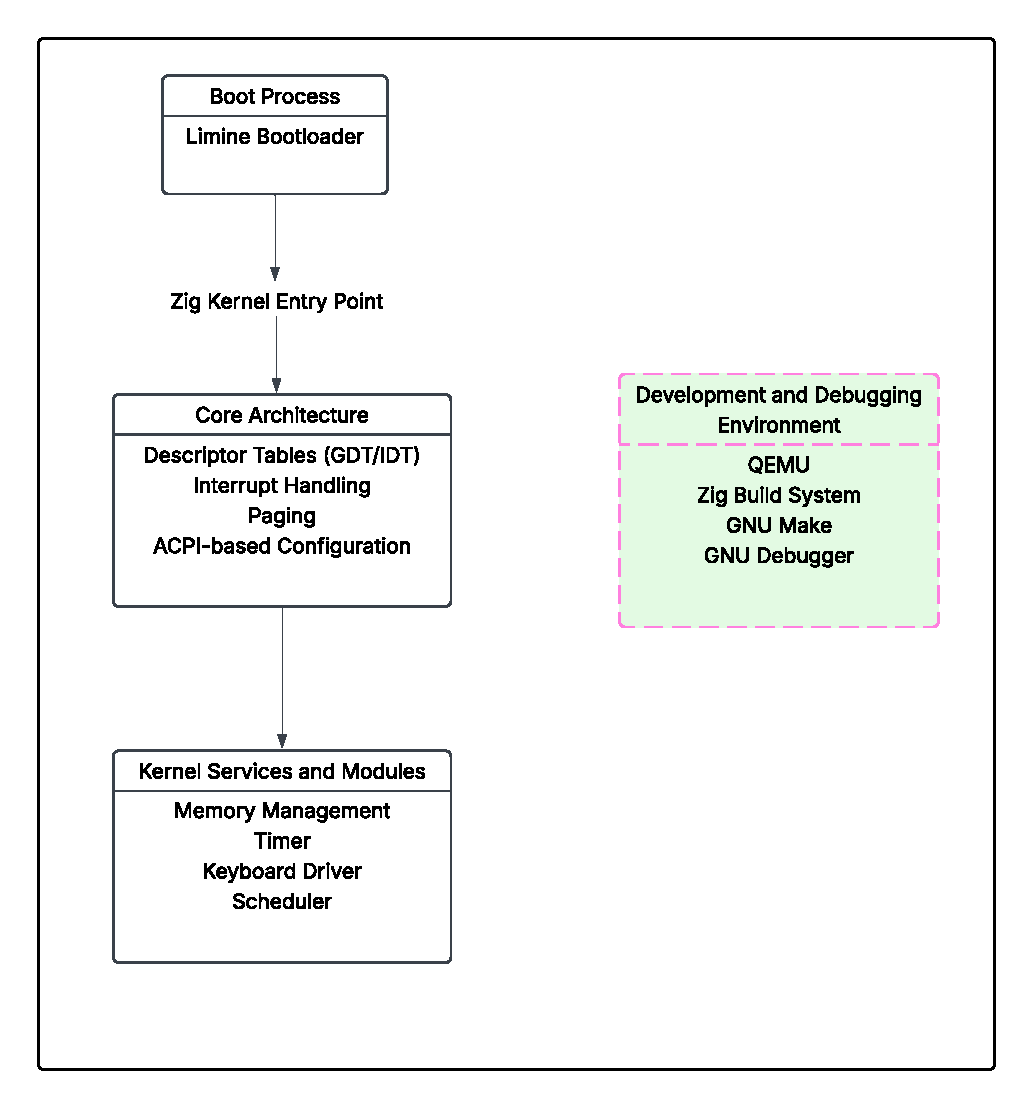
\includegraphics[width=0.9\textwidth]{figures/Architecture.pdf}
    \caption{Technical Architecture}
    \label{fig:Technical Architecture}
\end{figure}

On top of this core, various dependent modules are constructed—such as hardware
timers (PIT/HPET), keyboard drivers, a scheduler, system call interfaces, and a
simple in-memory file system. This modular design ensures that once the
architecture is stable, higher-level components can be built independently and
incrementally.

The development environment includes cross-compilation toolchains, QEMU for
virtualization, and framebuffer or serial output for debugging. All modules are
compiled into a monolithic kernel binary, which is deployed using the Limine
boot protocol.
\pagebreak

\subsection{Class Diagram}
The class diagram below illustrates the structural organization of KernelZ. It outlines the key components such as the Bootloader, CPU, memory managers, device drivers, and the Scheduler, each essential to the system's overall functionality.

\begin{figure}[h]
    \centering
    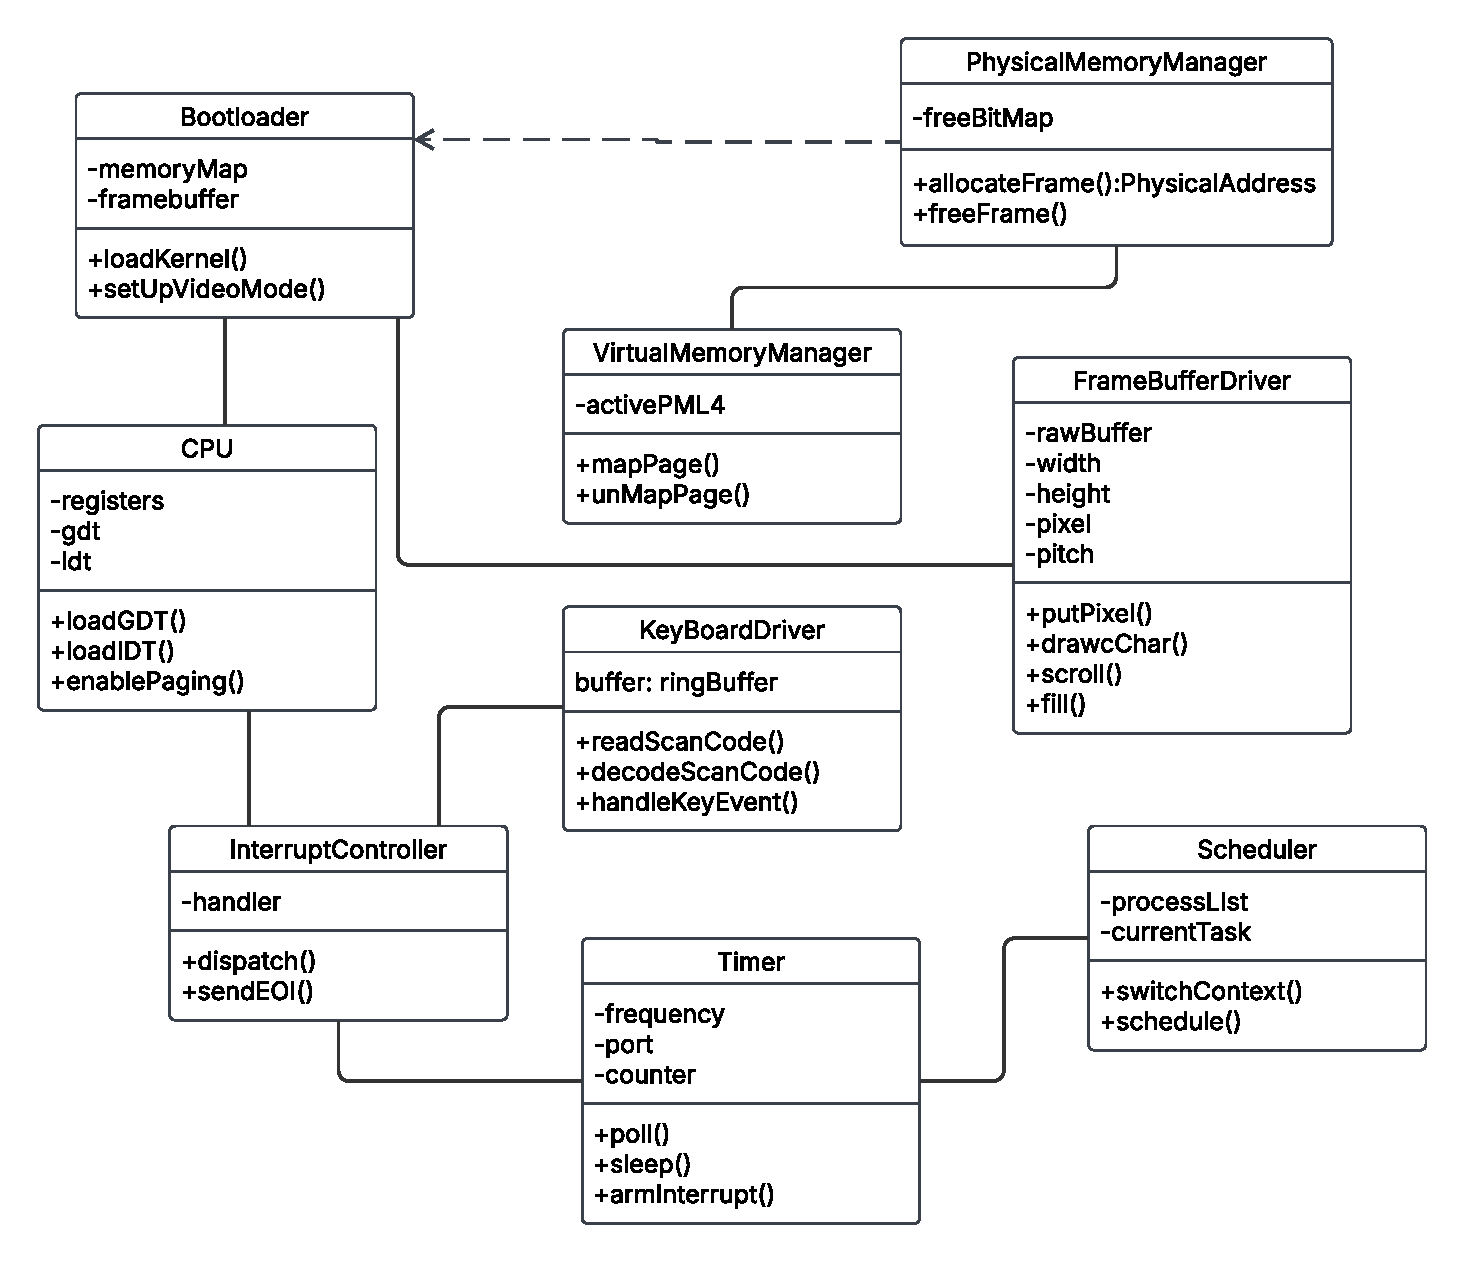
\includegraphics[width=\textwidth]{figures/class.pdf}
    \caption{Class Diagram}
    \label{fig:class_diagram}
\end{figure}

Each class is defined with relevant attributes and operations that describe its responsibilities. The diagram reflects how these components collaborate to handle memory management, interrupt processing, task scheduling, and hardware interaction within KernelZ.
\pagebreak




\pagebreak  

\subsection{Virtual to Physical Address Translation}

In x86\_64 long mode, virtual addresses are 64 bits wide, but only the lower 48 bits are used for addressing. The upper 16 bits (bits 63--48) must be a sign-extension of bit 47, forming a canonical address. The translation from virtual to physical address is performed by a four-level paging mechanism using 4 KiB pages.

\begin{table}[h]
    \renewcommand{\arraystretch}{1.5} % Increases row height
    \centering
    \begin{tabular}{|c|c|c|c|c|c|}
        \hline
        \textbf{Bits} & 47--39 & 38--30 & 29--21 & 20--12 & 11--0 \\
        \hline
        \textbf{Field} & PML4 Index & PDPT Index & PD Index & PT Index & Page Offset \\
        \hline
    \end{tabular}
    \caption{Virtual Address Field Breakdown}
    \label{tab:va_field_breakdown}
\end{table}

\vspace{1em}
\noindent\textbf{Translation Steps}\par
\vspace{0.5em}

The virtual address translation process is performed through a four-level paging hierarchy as shown in Figure~\ref{fig:virt-to-phys-map}.

\begin{figure}[H]
    \centering
    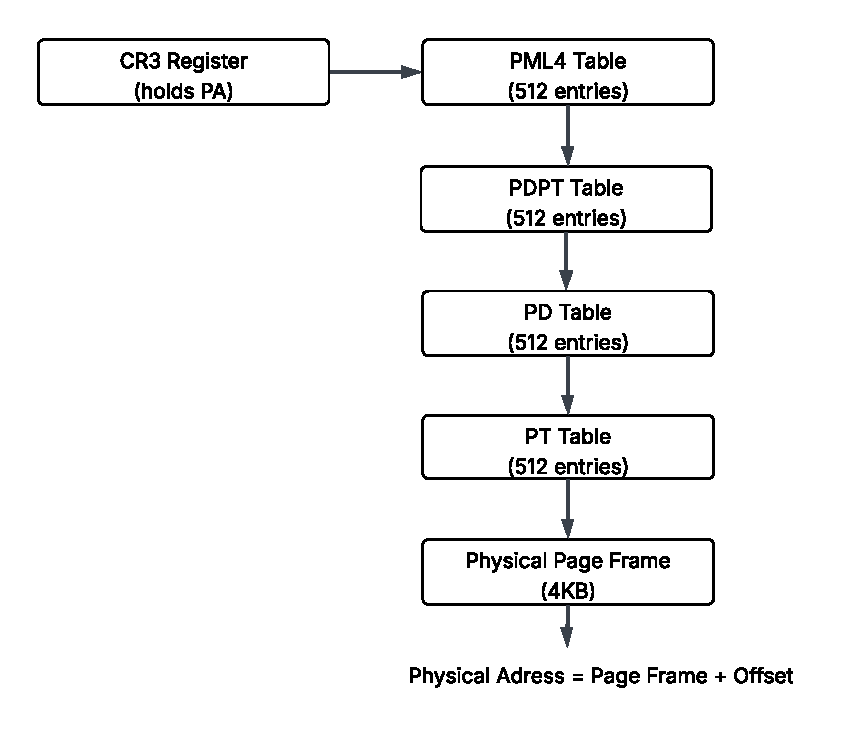
\includegraphics[width=\textwidth]{figures/VirtualToPhyMap.pdf}
    \caption{Virtual to Physical Memory Mapping}
    \label{fig:virt-to-phys-map}
\end{figure}
\begin{enumerate}
    \item \textbf{CR3 Register:} Holds the physical address of the base of the PML4 table (also called the Page Map Level 4).
    
    \item \textbf{PML4 Lookup:} Use bits 47--39 of the virtual address to index into the PML4 table. Each entry is 64 bits wide and contains the physical address of a Page Directory Pointer Table (PDPT).

    \item \textbf{PDPT Lookup:} Use bits 38--30 to index into the PDPT obtained from the PML4 entry. The selected entry gives the physical address of a Page Directory (PD).

    \item \textbf{PD Lookup:} Use bits 29--21 to index into the PD. This entry points to a Page Table (PT).

    \item \textbf{PT Lookup:} Use bits 20--12 to index into the PT. This entry points to the base physical address of a 4 KiB page frame.

    \item \textbf{Offset:} Bits 11--0 are the offset within the 4 KiB page. Add this to the page frame address to get the final physical address.
\end{enumerate}

\textbf{Final Calculation}
\begin{equation*}
\text{Physical Address} = \text{Page Frame Address} + \text{Offset}
\end{equation*}
\pagebreak

\subsection{Framebuffer and Terminal}

The text rendering system is responsible for displaying readable output during boot and kernel runtime. It is composed of two major components: the framebuffer and the terminal. The framebuffer interacts directly with memory-mapped video memory for pixel-level manipulation, while the terminal uses it to render structured, formatted text via a fixed-width bitmap font.

\subsubsection*{Purpose}
\begin{itemize}
    \item Enable early-stage screen output through a memory-mapped framebuffer.
    \item Support text rendering using a bitmap font and structured character grid.
    \item Handle formatted text output, scrolling, and cursor management.
\end{itemize}

\subsubsection*{System Flow}
\begin{enumerate}
    \item Limine bootloader provides framebuffer address, resolution, and pitch.
    \item The framebuffer is initialized using this metadata and a font is loaded.
    \item The terminal calculates screen dimensions in characters and prepares cursor state.
    \item Kernel logs and debug messages are printed using \texttt{print()}, rendering characters via the font glyphs.
\end{enumerate}

\subsubsection*{Framebuffer Module}

\begin{itemize}
    \item \textbf{Structure:} Defines the main framebuffer abstraction holding display memory and rendering metadata.
    \begin{lstlisting}[language=zig, breaklines=true, basicstyle=\ttfamily\footnotesize]
pub const Framebuffer = struct {
    buffer: []volatile Pixel,
    width: usize,
    height: usize,
    pixelWidth: usize,
    pitch: usize,
    font: Terminus,
};
    \end{lstlisting}

    \item \textbf{Initialization:}
    \begin{lstlisting}[language=zig, breaklines=true, basicstyle=\ttfamily\footnotesize]
pub fn init(fb_resp: *limine.FramebufferResponse) Error!Framebuffer
    \end{lstlisting}
    Uses bootloader information to map the video memory, calculate pixel layout, and load font data.

    \item \textbf{Screen Fill Operation:}  
    Sets all framebuffer pixels to a given color, useful for clearing the screen.
    \begin{lstlisting}[language=zig, breaklines=true, basicstyle=\ttfamily\footnotesize]
pub fn fill(self: Framebuffer, color: Color) void {
    @memset(self.buffer, color.toPixel());
}
    \end{lstlisting}

    \item \textbf{Scrolling Function:}
    \begin{lstlisting}[language=zig, breaklines=true, basicstyle=\ttfamily\footnotesize]
pub fn scroll(self: Framebuffer, bg_color: Color) void
    \end{lstlisting}
    Moves pixel data up by one text row and clears the last row to maintain terminal-like behavior.
\end{itemize}

\subsubsection*{Terminal Module}

\begin{itemize}
    \item \textbf{Initialization:}
    \begin{lstlisting}[language=zig, breaklines=true, basicstyle=\ttfamily\footnotesize]
pub fn init(raw_fb: *limine.FramebufferResponse, fg: Color, bg: Color) TtyError!void
    \end{lstlisting}
    Initializes framebuffer, computes the number of character rows and columns, and clears the screen.

    \item \textbf{Cursor and Wrapping:}  
    Maintains a cursor index and wraps text to the next line when it reaches the screen boundary. If the bottom is reached, it calls \texttt{scroll()}.

    \item \textbf{Formatted Output:}  
    Main function to render formatted strings using Zig’s formatting utilities.
    \begin{lstlisting}[language=zig, breaklines=true, basicstyle=\ttfamily\footnotesize]
pub fn print(comptime fmt: []const u8, args: anytype) TtyError!void {
    std.fmt.format(writer, fmt, args) catch return TtyError.PrintError;
}
    \end{lstlisting}
    Converts characters into glyphs and draws them to the framebuffer via the writer interface.
\end{itemize}

This layered rendering system ensures that KernelZ has robust, structured output capability during boot and runtime. The framebuffer provides raw pixel access, while the terminal abstracts it into a text-based interface with scrolling, cursor control, and formatted printing.
\pagebreak

\subsection{Physical Memory Manager (PMM)}

The Physical Memory Manager (PMM) is the foundational component in the memory subsystem. It is responsible for managing physical RAM by dividing it into fixed-size blocks called \textit{frames} (each 4\,KiB in size) and tracking their availability using a bitmap. All other memory-related features—such as paging, heap allocation, and virtual memory management are built on top of the PMM.

\subsubsection*{Purpose and Role}

The PMM enables the kernel to:
\begin{itemize}
  \item Detect usable memory provided by the bootloader via the Limine memory map.
  \item Allocate and deallocate physical memory frames safely and efficiently.
  \item Prevent memory corruption by avoiding reuse of reserved memory regions (e.g., kernel code, page tables, framebuffer).
\end{itemize}

This system ensures deterministic and predictable memory behavior, which is essential in low-level kernel development.

\subsubsection*{Initialization Process (\texttt{init()})}

During early boot, the kernel executes the PMM initialization routine. The steps involved are:

\begin{enumerate}
  \item \textbf{Receive Memory Map from Limine:} The bootloader provides a memory map indicating memory regions and their types (USABLE, RESERVED, FRAMEBUFFER, etc.).
  
  \item \textbf{Parse Usable Regions:} The kernel scans this map to identify USABLE memory ranges available for allocation.
  
  \item \textbf{Calculate Total Frames and Allocate Bitmap:} Physical memory is divided into 4\,KiB frames. A single bit in the bitmap represents each frame. For instance, 1\,GiB of RAM results in 262,144 frames, needing a 32,768-byte (256\,KiB) bitmap.
  
  \item \textbf{Mark Reserved Regions:} The bitmap marks certain regions as used to avoid accidental reuse:
    \begin{itemize}
      \item Kernel ELF sections (\texttt{.text}, \texttt{.data}, \texttt{.bss})
      \item Limine boot structures
      \item Framebuffer memory
      \item Page tables and kernel stack
    \end{itemize}
\end{enumerate}

\subsubsection*{Core Functions}

\textbf{\texttt{allocateFrame()}}  
\begin{itemize}
  \item Scans the bitmap for the first unset bit (0), sets it to used (1).
  \item Returns the physical address using:
  \[
  \texttt{phys\_addr} = \texttt{frame\_index} \times \texttt{PAGE\_SIZE}
  \]
\end{itemize}

\textbf{\texttt{freeFrame(phys\_addr)}}  
\begin{itemize}
  \item Converts a physical address to frame index and clears the corresponding bit:
  \[
  \texttt{frame\_index} = \frac{\texttt{phys\_addr}}{\texttt{PAGE\_SIZE}}
  \]
\end{itemize}

This mechanism ensures fast and lightweight frame management.

\subsubsection*{Internal Working Flow}
The Physical Memory Manager's operation begins during the kernel initialization phase, right after the bootloader transfers control. At this stage, the kernel receives a memory map from Limine and uses it to identify which regions of RAM are usable. These regions are broken down into fixed-size 4\,KiB frames, and a bitmap is created to track their usage status. Each bit in the bitmap corresponds to a single frame — a 0 indicates that the frame is free, and a 1 marks it as allocated.
\begin{figure}[H]
    \centering
    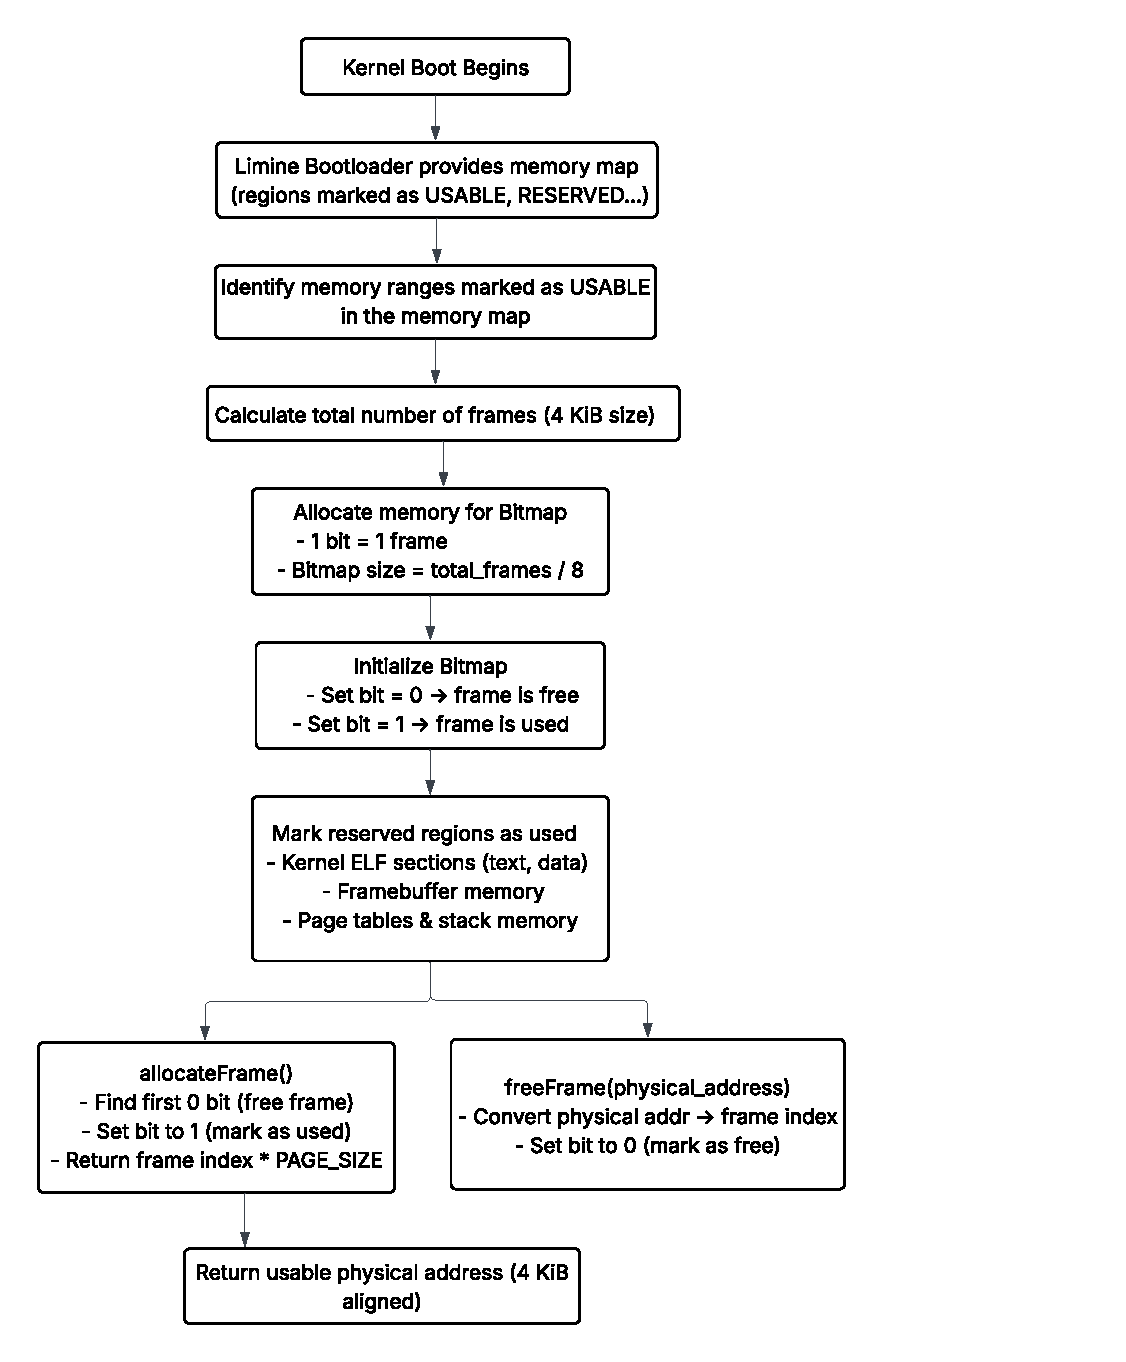
\includegraphics[width=1.1\linewidth]{figures/Physical Memory Manager.pdf}
    \caption{Physical Memory Manager}
    \label{fig:Physical Memory Manager}
\end{figure}

Once the bitmap is allocated and initialized, the kernel marks memory regions it already uses (such as the kernel image, stack, page tables, and framebuffer) as reserved. From this point onward, frame allocations and deallocations can be handled dynamically using two core functions: \texttt{allocateFrame()}, which returns a free frame, and \texttt{freeFrame()}, which marks a previously allocated frame as available again.
\subsubsection*{Example Usage}

\begin{lstlisting}
const frame = PhysicalMemoryManager.allocateFrame();
Paging.mapPage(virtual_addr, frame);
\end{lstlisting}

\subsubsection*{Error Handling and Safety}

If no free frame is available, \texttt{allocateFrame()} returns \texttt{null}, enabling the kernel to handle memory exhaustion gracefully. Future improvements may include double-free detection and boundary checks to ensure robustness.
\pagebreak

\subsection{Paging Subsystem Implementation}

The Paging subsystem in \textbf{KernelZ} is responsible for establishing and manipulating page table structures used to translate virtual addresses to physical memory addresses. It interacts with the Physical Memory Manager (PMM) to allocate frames for each page table level and supports flexible APIs for memory mapping and unmapping.

The logical structure of paging and how a virtual address is broken down into page table indices is already discussed in Section~\ref{tab:va_field_breakdown} and Figure~\ref{fig:virt-to-phys-map}. This section focuses on the implementation of paging functions and the memory translation process.


The logical structure of paging and how a virtual address is broken down into page table indices are already discussed in Section~\ref{tab:va_field_breakdown} and Figure~\ref{fig:virt-to-phys-map}. This section focuses on the actual code-level implementation of mapping, unmapping, and managing virtual memory regions through hierarchical page tables.

\subsubsection*{Purpose}

\begin{itemize}
  \item Build virtual memory abstraction over physical RAM.
  \item Maintain and modify multi-level page tables in x86\_64.
  \item Provide mapping and unmapping APIs for virtual memory setup.
  \item Enable higher-half kernel and dynamic heap/VMM memory regions.
\end{itemize}

\subsubsection*{Key Implementation Functions}

\vspace{0.5em}
\noindent\textbf{\texttt{mapPage(virt\_addr, phys\_addr, flags)}}
\begin{itemize}
  \item Extract PML4, PDPT, PD, PT indices from \texttt{virt\_addr}.
  \item Walk page tables starting from CR3 (PML4 base).
  \item At each level, if entry is missing:
  \begin{itemize}
    \item Request a physical frame from PMM.
    \item The frame is zeroed and its address is inserted into the parent table with flags.
  \end{itemize}
  \item At PT level, write:
  \texttt{entry = phys\_addr | flags}.
  \item Optionally flush TLB using \texttt{invlpg}.
\end{itemize}

\noindent\textbf{Flags commonly used:}
\begin{itemize}
  \item \texttt{Present} (bit 0): Page is mapped.
  \item \texttt{Writable} (bit 1): Allows write access.
  \item \texttt{User-accessible} (bit 2): Optional, for future userspace.
\end{itemize}

\vspace{0.5em}
\noindent\textbf{\texttt{mapRange(start\_virt, start\_phys, page\_count, flags)}}
\begin{itemize}
  \item Iteratively maps multiple 4\,KiB pages using \texttt{mapPage()}.
  \item Ensures alignment and batching for performance.
  \item Used during kernel ELF mapping, heap region setup, identity mappings.
\end{itemize}

\vspace{0.5em}
\noindent\textbf{\texttt{unmapPage(virt\_addr)}}
\begin{itemize}
  \item Locates the page table entry at PT level.
  \item Sets entry to 0 and calls \texttt{invlpg} to flush TLB.
\end{itemize}

\vspace{0.5em}
\noindent\textbf{\texttt{unmapRange(start\_virt, page\_count)}}
\begin{itemize}
  \item Clears mappings of multiple pages.
  \item Checks for entry presence before unmapping.
  \item Does not immediately free page tables.
\end{itemize}

\subsubsection*{Page Table Entry Flags}

Each page table entry not only holds the physical address of the next-level table or data page, but also includes a set of control flags. These flags play a crucial role in defining how the memory can be accessed, whether it is readable, writable, user-accessible, or cacheable. The correct use of these flags is critical to enforcing memory protection, isolating the kernel and user space, and optimizing performance.

\begin{table}[H]
\centering
\begin{tabular}{|c|l|l|}
\hline
\textbf{Bit} & \textbf{Name} & \textbf{Description} \\
\hline
0 & Present & Page is resident in memory \\
1 & Writable & 1 = Writable, 0 = Read-only \\
2 & User & 1 = Accessible from ring 3 (optional) \\
3 & Write-through & Enable write-through caching \\
4 & Cache Disable & Disable CPU caching \\
7 & Page Size & 1 = Large (2\,MiB/1\,GiB), 0 = 4\,KiB \\
\hline
\end{tabular}
\caption{Page Table Entry Flags}
\end{table}

\subsubsection*{Unmapping and TLB Consistency}
\begin{itemize}
  \item TLB entries must be flushed after unmapping to avoid stale translations.
  \item \texttt{invlpg} is used to flush a specific page.
  \item Page tables themselves are not freed immediately to simplify memory reuse.
\end{itemize}
\vspace{1em}
\noindent
In summary, the Paging subsystem in KernelZ bridges the gap between abstract virtual memory and real physical memory. It allows flexible and secure memory layout by dynamically mapping and unmapping pages. By interfacing tightly with the Physical Memory Manager and supporting higher-half kernel mappings, it forms the backbone of virtual memory infrastructure required by both the Virtual Memory Manager and Heap Allocator.
\pagebreak


\subsection{Virtual Memory Manager (VMM)}

The Virtual Memory Manager (VMM) acts as the abstraction layer over paging. It is responsible for managing dynamic allocation and reservation of virtual memory regions. It allows the kernel to request memory safely, flexibly, and independently of the physical layout. While paging performs the actual virtual-to-physical address translation, the VMM determines where and how memory is mapped to support the kernel heap, stacks, subsystems, and future userspace regions.

\subsubsection*{Purpose}

The VMM enables the kernel to:
\begin{itemize}
  \item Reserve arbitrary-length virtual address regions in the higher-half kernel address space.
  \item Dynamically map physical memory to those regions via paging.
  \item Manage metadata using lightweight structures called \texttt{VmObject}s.
  \item Track virtual memory allocations to allow unmapping and region cleanup.
  \item Provide a foundation for the kernel heap and eventually userspace VMM instances.
\end{itemize}

\subsubsection*{Key Structures}

\paragraph{VmObject} 

\texttt{VmObject} represents a continuous reserved region of virtual memory. It contains the following fields:
\begin{itemize}
  \item \texttt{start\_addr}: Base virtual address of the region.
  \item \texttt{page\_count}: Number of 4\,KiB pages in the region.
  \item \texttt{flags}: Memory access permissions (read, write, execute).
\end{itemize}

Each \texttt{VmObject} is stored in a dynamic list maintained by the VMM and is allocated using Zig’s \texttt{FixedBufferAllocator}.

\paragraph{vmm\_heap.zig}

This module initializes a custom allocator used to allocate internal metadata like \texttt{VmObject}s. It is used only within the VMM to prevent dependency cycles with the kernel heap.

\subsubsection*{Core Functions}

\noindent\textbf{\texttt{reserveRange(page\_count: usize) -> *VmObject}}  
\begin{itemize}
  \item Finds a free virtual address range large enough to accommodate \texttt{page\_count} pages.
  \item Does not allocate physical memory.
  \item Allocates and returns a \texttt{VmObject} to track this reservation.
\end{itemize}

\noindent\textbf{\texttt{mapRange(vm\_obj: *VmObject, phys\_start: usize, flags)}}  
\begin{itemize}
  \item Maps each page in the \texttt{VmObject} to physical memory starting from \texttt{phys\_start}.
  \item Uses \texttt{Paging.mapPage()} to perform mappings.
  \item Supports various flags, such as writable, executable, and MMIO-mapped.
\end{itemize}

\noindent\textbf{\texttt{unmapRange(vm\_obj: *VmObject)}}  
\begin{itemize}
  \item Walks through the virtual region described in \texttt{VmObject} and unmaps each page.
  \item Uses \texttt{Paging.unmapPage()} to perform unmapping.
  \item Frees the associated metadata and returns the address range to the available pool.
\end{itemize}

\subsubsection*{Working Flow – Virtual Memory Reservation and Mapping}

\noindent
The general flow of virtual memory management is as follows:
\begin{enumerate}
  \item Call \texttt{reserveRange(n)} to find and reserve a region of virtual memory.
  \item The VMM searches for a free virtual address block in the higher-half space.
  \item It allocates a \texttt{VmObject} using its internal allocator.
  \item \texttt{mapRange()} is called to map physical pages into the virtual region.
  \item The pages are then usable by higher-level kernel code.
\end{enumerate}

\subsubsection*{Integration with Other Components}

\begin{table}[H]
\centering
\begin{tabular}{|l|p{10cm}|}
\hline
\textbf{Component} & \textbf{Role in VMM Workflows} \\
\hline
\texttt{PhysicalMemoryManager} & Supplies physical frames to be mapped during \texttt{mapRange()}. \\
\texttt{Paging} & Maps and unmaps individual pages for \texttt{mapRange()} and \texttt{unmapRange()}. \\
\texttt{Heap Allocator} & Built on top of VMM; uses \texttt{reserveRange()} to acquire virtual memory. \\
\texttt{vmm\_heap.zig} & Internal allocator used to allocate metadata such as \texttt{VmObject}s. \\
\hline
\end{tabular}
\caption{Integration of VMM with Other Kernel Components}
\label{tab:vmm_components}
\end{table}



\subsubsection*{Memory Protection}

All virtual memory regions managed by the VMM carry access flags, which are enforced by the underlying page tables during memory access. These flags define access permissions for each region.

Future extensions may include:
\begin{itemize}
  \item User/supervisor separation to support user-mode isolation.
  \item Executable-only pages for safe code execution.
  \item MMIO-specific mappings with uncached access properties.
\end{itemize}



The Virtual Memory Manager provides a structured abstraction over paging by enabling memory reservation, mapping, and metadata tracking. It forms the basis for dynamic memory management in the kernel, supporting flexible and safe memory layouts. By separating reservation and mapping logic, the VMM supports efficient reuse of memory regions and prepares the kernel for future userspace memory management capabilities.
\pagebreak
\subsection{Heap Allocator}

To support dynamic memory allocation during kernel execution, a custom heap allocator was implemented in Zig. The allocator operates atop the Virtual Memory Manager (VMM), which in turn is backed by the Physical Memory Manager (PMM). This layered design allows KernelZ to efficiently service variable-sized allocation requests from different kernel components such as the scheduler, driver subsystems, and internal data structures.

\subsubsection*{Purpose and Role}

The heap allocator provides a general-purpose, dynamic memory facility for kernel code. Its key responsibilities are:

\begin{itemize}
    \item Efficiently allocate and free memory of arbitrary size at runtime.
    \item Reuse freed memory to reduce fragmentation and memory pressure.
    \item Expand the heap when no suitable block is available using virtual memory mechanisms.
    \item Abstract low-level frame management details from higher-level kernel services.
\end{itemize}

It acts as the default backend for dynamic allocations in the kernel, enabling flexible memory usage during system operation.

\subsubsection*{Heap Structure and Metadata}

The heap is modeled as a \textbf{doubly linked list} of nodes, where each node represents a contiguous chunk of heap memory. Each node carries the following metadata:

\begin{lstlisting}[breaklines=true, basicstyle=\ttfamily\footnotesize]
const HeapNode = struct {
    size: usize,             // Size of this block (excluding header)
    status: u8,              // Used (1) or Free (0)
    prev: ?*HeapNode,        // Pointer to previous node
    next: ?*HeapNode,        // Pointer to next node
};
\end{lstlisting}

Each allocation includes overhead equivalent to \texttt{@sizeOf(HeapNode)} and is aligned to platform word size (typically 8 or 16 bytes). Nodes marked as free are eligible for reuse.

\subsubsection*{Allocation Algorithm}

When \texttt{alloc(size)} is called:

\begin{itemize}
    \item The allocator scans the heap list to locate the first free node with \texttt{size >= requested\_size}.
    \item If found:
    \begin{itemize}
        \item The node is used directly or \textbf{split} if the remaining size is large enough to hold a new \texttt{HeapNode}.
        \item The selected node is marked as used, and a pointer to the memory region immediately after the header is returned.
    \end{itemize}
    \item If no suitable node is found, a new node needs to be carved out from the end of the heap. However, if the new node to be carved out exceeds the boundaries of the current heap, the heap is \textbf{expanded} by requesting a new larger region from the underlying VMM.
\end{itemize}

This strategy uses a \textbf{first-fit} policy to balance simplicity and speed in early kernel operation.

\subsubsection*{Deallocation and Coalescing}

The \texttt{free(ptr)} function marks a block as free and attempts to merge with adjacent free blocks to reduce fragmentation.

\begin{itemize}
    \item It checks both \texttt{prev} and \texttt{next} neighbors for free status.
    \item If either is free, their sizes are merged, and the list is updated accordingly.
\end{itemize}

This coalescing approach improves the likelihood of satisfying future large allocation requests.

\subsubsection*{Example Workflow}

\begin{lstlisting}[breaklines=true, basicstyle=\ttfamily\footnotesize]
const a = heap.alloc(64);   // allocates 64 bytes
const b = heap.alloc(32);   // allocates 32 bytes
heap.free(a);               // frees first block
const c = heap.alloc(48);   // reuses or splits the freed block
\end{lstlisting}

If \texttt{b} is freed later, the allocator will merge adjacent free blocks into one larger region.

\subsubsection*{Integration with VMM and PMM}

\begin{table}[H]
\centering
\begin{tabular}{|l|p{10cm}|}
\hline
\textbf{Component} & \textbf{Role} \\
\hline
VMM & Reserves and maps heap regions. \\
PMM & Provides physical frames backing the mapped regions. \\
Paging & Enforces access protection and memory isolation. \\
\hline
\end{tabular}
\caption{Heap Allocator Integration with Memory Subsystems}
\end{table}

All heap memory resides in the kernel address space, typically starting just after the kernel binary in the higher-half virtual layout (e.g., \texttt{0xFFFFFFFF80006000}).

\subsubsection*{Current Limitations}

\begin{itemize}
    \item Does not support slab allocation strategies incurring greater memory overhead due to inline metadata and linked list usage.
    \item Not thread-safe; assumes a single-core or preemption-disabled context.
    \item Allocation is linear time (\texttt{O(n)} worst case).
\end{itemize}

\pagebreak
\subsection{Memory Management Architecture}
Figure~\ref{fig:memory-management} outlines the flow of memory allocation and translation within KernelZ. The memory management subsystem is modular, handling both physical and virtual memory, and is built around a clean abstraction between kernel/user space.
\begin{figure}[H]
    \centering
    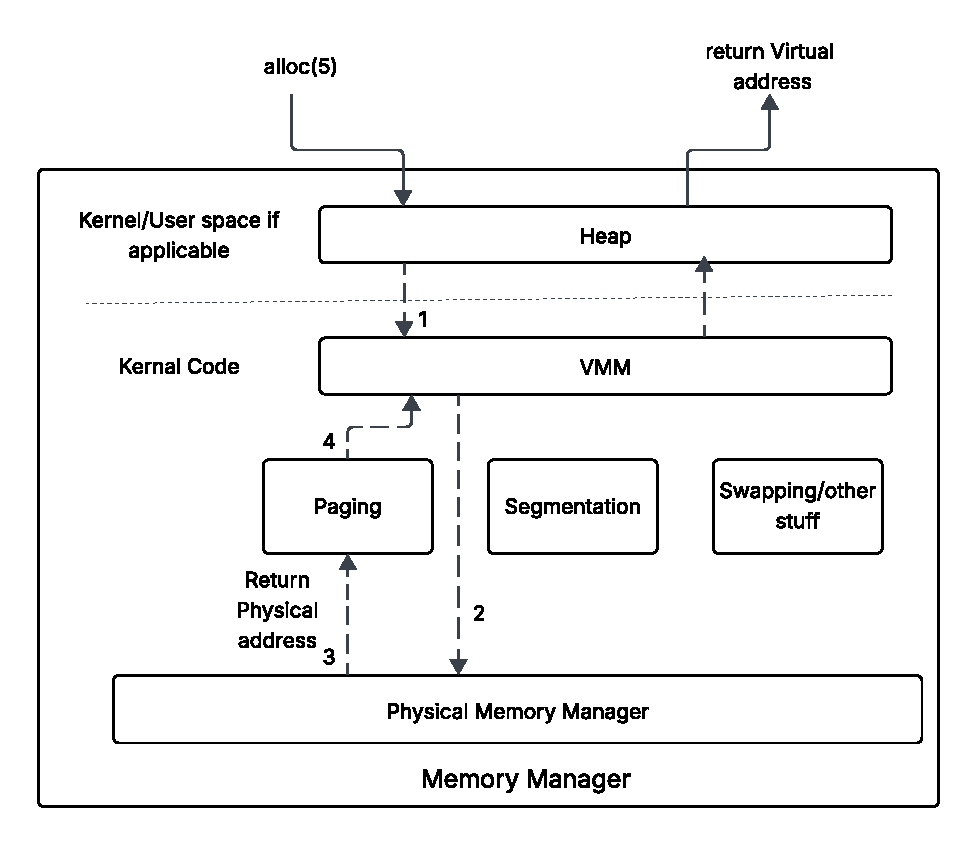
\includegraphics[width=0.8\textwidth]{figures/Memory Management.pdf}
    \caption{Memory Management Workflow}
    \label{fig:memory-management}
\end{figure}

\begin{enumerate}
    \item \textbf{alloc(n)}: A request to allocate memory of size \texttt{n} bytes is issued by the kernel or higher-level subsystems.
    \item \textbf{Virtual Address Return}: The memory manager returns a virtual address through the virtual memory allocator (VMM), often backed by paging.
    \item \textbf{Virtual-to-Physical Mapping}: The virtual address is translated into a physical address using page tables managed by the kernel.
    \item \textbf{Physical Allocation}: The physical memory manager (PMM) is responsible for allocating physical frames from free memory and returning the mapped physical address.
\end{enumerate}



\subsubsection*{Subsystem Breakdown}

\begin{itemize}
    \item \textbf{Memory Manager}: Central unit coordinating allocation, tracking usage, and enforcing kernel/user space boundaries.
    \item \textbf{Physical Memory Manager (PMM)}: Handles actual memory pages; maintains a bitmap of free/used frames.
    \item \textbf{Virtual Memory Manager (VMM)}: Implements paging - translating virtual addresses to physical - creating the necessary page tables.
    \item \textbf{Heap Manager}: Dynamically provides allocations via \texttt{alloc()} and possibly \texttt{free()} interface, built atop VMM.
\end{itemize}

\subsubsection*{Optional Features}

\begin{itemize}
    \item \textbf{Paging}: GDT segments and page tables manage memory protection and isolation. Kernel resides in higher-half mapping.
    \item \textbf{Swapping/Other}: While not implemented yet, support for swapping or out-of-core mechanisms can be added later.
    \item \textbf{Kernel/User Space Split}: If userspace is supported, memory protection and isolation mechanisms become crucial.
\end{itemize}
\pagebreak


\subsection{Timer}

\subsubsection*{Introduction}

Accurate timekeeping and interrupt scheduling are critical in any operating system kernel. KernelZ supports multiple hardware timer sources including the Programmable Interval Timer (PIT), High Precision Event Timer (HPET), Local APIC Timer (LAPIC), and Time Stamp Counter (TSC). Each timer is initialized based on system capabilities and used for different purposes such as delay routines, context switching, and performance benchmarking.

\subsubsection*{Purpose}

\begin{itemize}
    \item Initialize and configure multiple hardware timers for system use.
    \item Use periodic and deadline-based timer interrupts for scheduling and delays.
    \item Abstract different hardware capabilities under a consistent interface.
\end{itemize}

\subsubsection*{Timer Initialization Flow}

\begin{enumerate}
    \item PIT is initialized early for basic delay and calibration.
    \item HPET or LAPIC is configured next if supported for more precise interrupts.
    \item TSC is calibrated against PIT or HPET and used as a high-resolution counter.
    \item Timer interrupts are routed to the kernel scheduler or delay subsystems.
\end{enumerate}

\subsubsection*{Programmable Interval Timer (PIT)}

\begin{itemize}
    \item \textbf{Purpose:} Provides basic periodic interrupts using legacy hardware (channel 0).
    
    \item \textbf{Initialization:}
    \begin{lstlisting}[language=zig]
    pub fn init() void
    \end{lstlisting}
    Configures PIT in mode 2 (rate generator) and sets a divisor for interrupt frequency.

    \item \textbf{Wait Function:}
    \begin{lstlisting}[language=zig]
    pub fn wait(ms: u64) void
    \end{lstlisting}
    Implements busy-wait delays by counting PIT ticks in a loop.
\end{itemize}

\subsubsection*{High Precision Event Timer (HPET)}

\begin{itemize}
    \item \textbf{Purpose:} Offers high-resolution and reliable periodic interrupts.
    
    \item \textbf{Structure:}
    \begin{lstlisting}[language=zig]
    pub const Hpet = struct {
        base: *volatile HpetRegisters,
        frequency: u64,
    };
    \end{lstlisting}

    \item \textbf{Initialization:}
    \begin{lstlisting}[language=zig]
    pub fn init(base: usize) Hpet
    \end{lstlisting}
    Maps the MMIO base address, disables legacy replacement mode, and enables timer.
\end{itemize}

\subsubsection*{Local APIC Timer (LAPIC)}

\begin{itemize}
    \item \textbf{Purpose:} Enables per-core timer interrupts and supports TSC deadline mode.

    \item \textbf{Initialization:}
    \begin{lstlisting}[language=zig]
    pub fn init(vector: u8) void
    \end{lstlisting}
    Configures the LAPIC timer LVT (Local Vector Table) with interrupt vector and periodic mode.

    \item \textbf{Set Timer Function:}
    \begin{lstlisting}[language=zig]
    pub fn setTimer(count: u32) void
    \end{lstlisting}
    Loads the LAPIC timer with the given tick count to trigger interrupt after that duration.
\end{itemize}

\subsubsection*{Time Stamp Counter (TSC)}

\begin{itemize}
    \item \textbf{Purpose:} Provides a CPU-cycle counter for high-precision timestamping and benchmarking.

    \item \textbf{Structure:}
    \begin{lstlisting}[language=zig]
    pub const TscTimer = struct {
        ticks_per_ms: u64,
    };
    \end{lstlisting}

    \item \textbf{Initialization:}
    \begin{lstlisting}[language=zig]
    pub fn init(vector: u8) TscTimer
    \end{lstlisting}
    Checks hardware support for TSC deadline, configures LAPIC to use TSC-deadline mode.

    \item \textbf{Set Deadline:}
    \begin{lstlisting}[language=zig]
    pub fn setDeadline(self: TscTimer, ms: u64) void
    \end{lstlisting}
    Computes the target TSC value and writes it to the MSR to trigger a deadline interrupt.
\end{itemize}


The timer subsystem  supports legacy and modern hardware interfaces for clock interrupts and scheduling. PIT and HPET provide foundational timing capabilities, while LAPIC and TSC enable advanced interrupt strategies such as per-core timers and deadline-based events. This flexible design allows the kernel to use the most precise and efficient timer available on the system.

\pagebreak

\subsection{Keyboard Handler Workflow}
The keyboard handler is a key part of the kernel's interrupt-driven input system. When a user presses or releases a key, the following steps occur as outlined in Figure~\ref{fig:keyboard-handler}.

\begin{figure}[H]
    \centering
    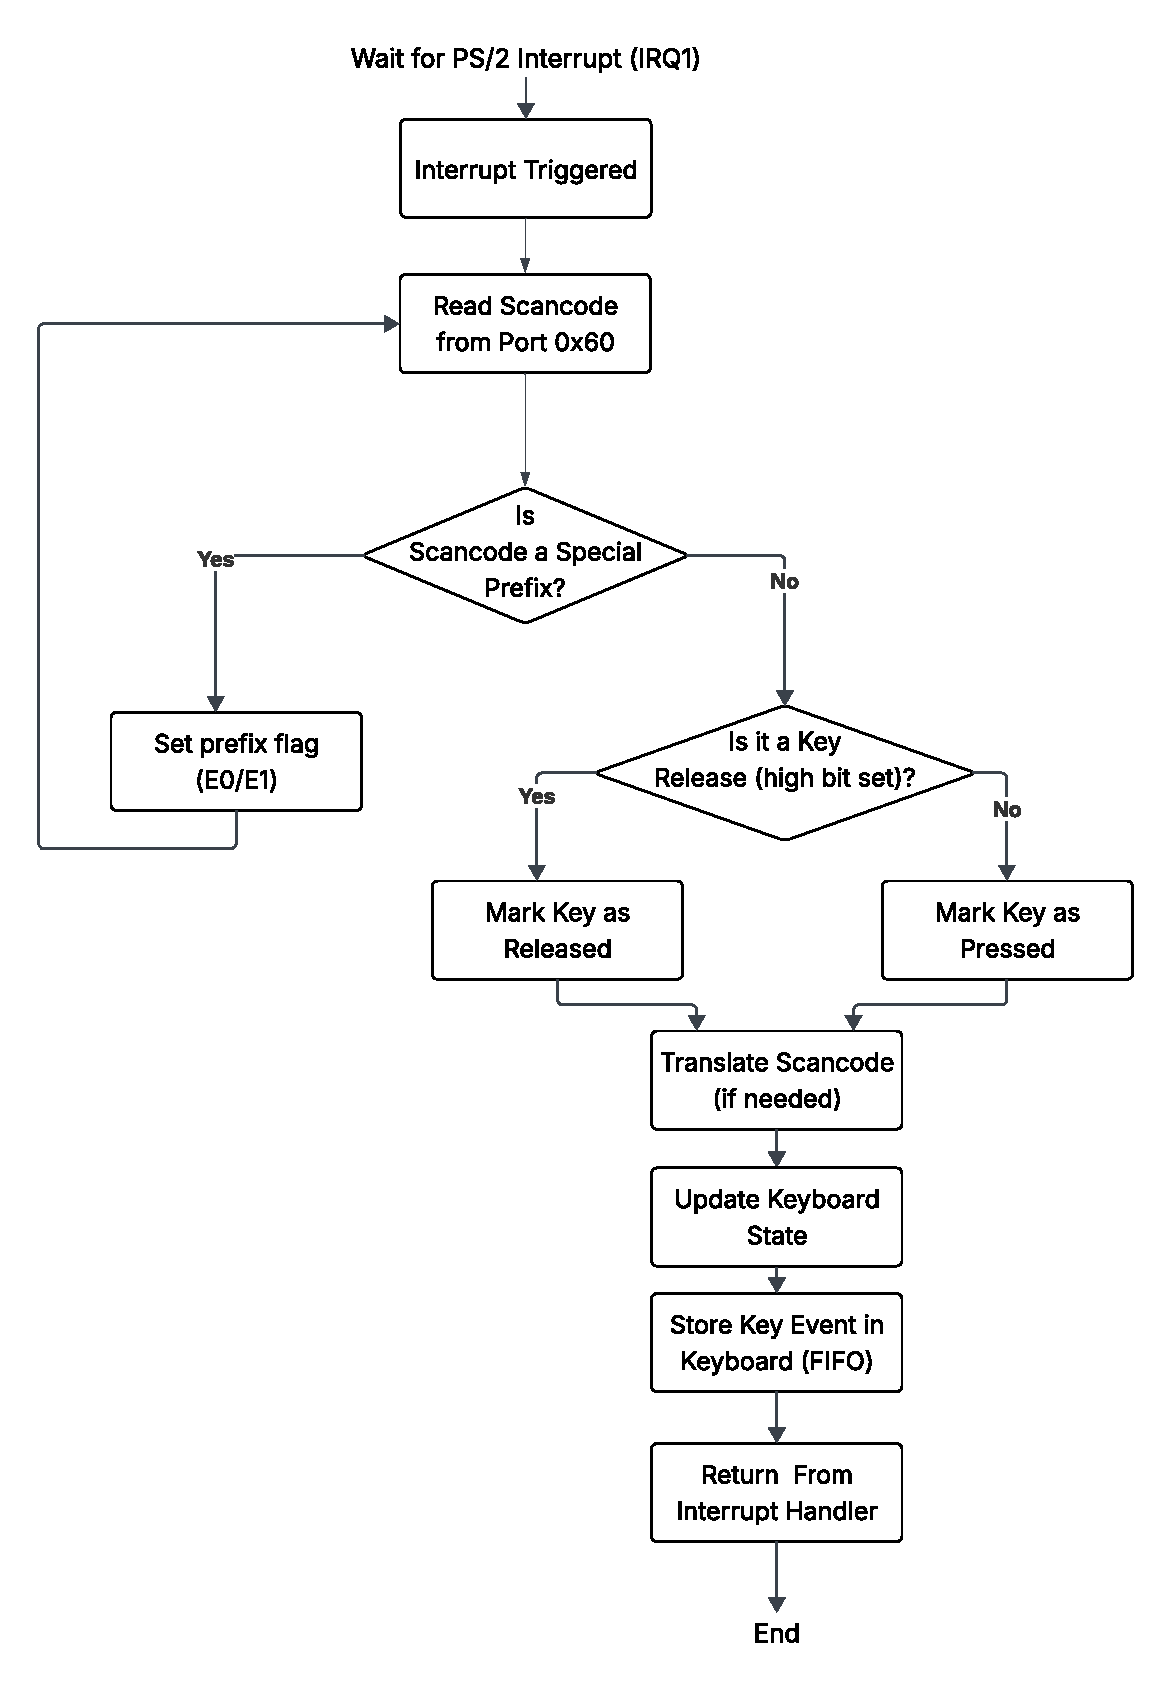
\includegraphics[width=0.8\linewidth]{figures/Keyboard Handler.pdf}
    \caption{Keyboard Handler}
    \label{fig:keyboard-handler}
\end{figure}
\begin{enumerate}
    \item \textbf{Interrupt Triggered}: IRQ1 is raised when a keyboard event occurs.
    \item \textbf{Read Scancode}: The PS/2 controller provides the scancode via I/O port \texttt{0x60}.
    \item \textbf{Special Prefix Check}: Certain keys begin with a prefix byte (e.g., \texttt{0xE0}). If found, the handler waits for the next byte to form a full scancode. When a prefix byte is encountered, the driver enters a prefix state, where the succeeding scancodes have different meanings than if they were encountered in the normal state.
    \item \textbf{Press or Release}: Based on the MSB of the scancode (for PS/2 Set 1), the key is marked as pressed or released.
    \item \textbf{Scancode Translation}: The raw code is translated to an ASCII character or symbolic key using a lookup table.
    \item \textbf{Update Keyboard State}: Modifier states (Shift, Ctrl, Alt) are updated to reflect current key states.
    \item \textbf{Store in FIFO}: The resulting event is pushed to a keyboard event FIFO buffer for use by other components, where each event also includes a status flag indicating the modifier states.
    \item \textbf{Return from Interrupt}: The handler finishes, and the interrupted instruction resumes.
\end{enumerate}

\subsubsection*{Optional Extensions}
To improve user interaction and support more features, the following extensions are implemented or planned:

\begin{itemize}
    \item \textbf{Handle Control Sequences}: Key combinations like \texttt{Ctrl+Alt+Del} are detected and mapped to system-level actions such as rebooting or triggering a kernel panic.
    \item \textbf{Non-Printable Keys}: Function keys (F1--F12), arrow keys, Insert/Delete, etc., are processed separately from printable characters to provide navigation or command functionality.
    \item \textbf{Multi-byte Sequences}: Certain key sequences modify the next input character (e.g., \^{} + e $\rightarrow$ ê), requiring the handler to buffer and combine inputs intelligently.
\end{itemize}
\pagebreak

\subsection{Interrupt Handling Workflow}
Figure~\ref{fig:interrupt_flow} outlines how KernelZ handles various interrupts, including hardware signals, exceptions, and spurious cases. It evaluates their type and origin, then either handles them, ignores them, or escalates to process termination or system panic before resuming execution with \texttt{IRET}.

\begin{figure}[H]
    \centering
    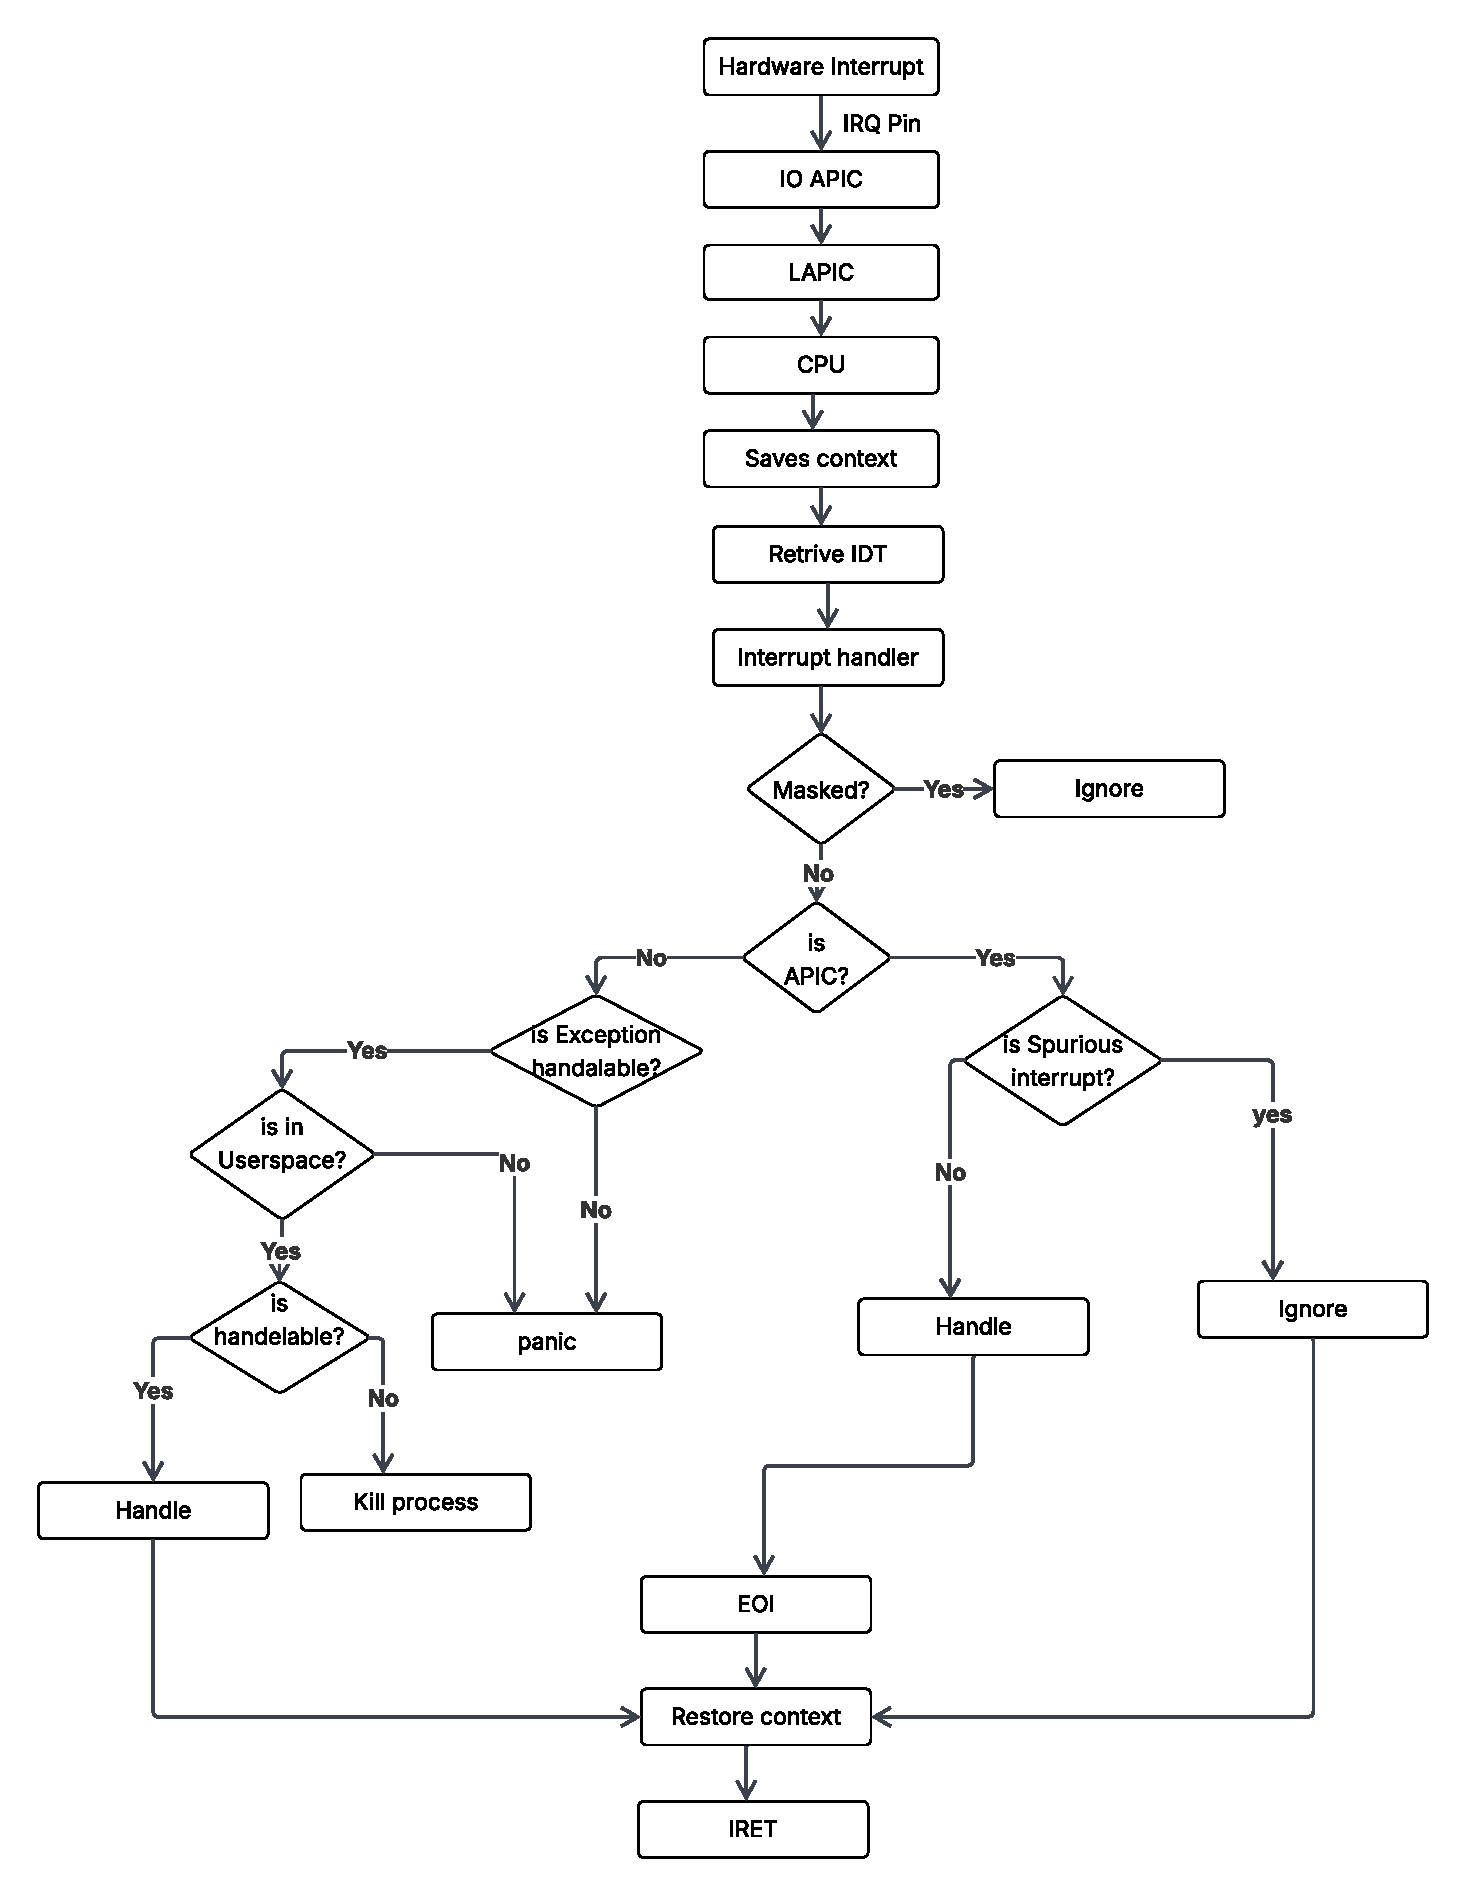
\includegraphics[width=0.9\textwidth]{figures/interrupt.pdf}
    \caption{Interrupt Handling Workflow}
    \label{fig:interrupt_flow}
\end{figure}
\pagebreak

\subsection{Scheduler}

The scheduler in KernelZ provides cooperative multitasking through a simple round-robin algorithm. It manages kernel-level threads called processes and switches between them on timer interrupts or through explicit yielding. The design ensures that there is always at least one process (usually the idle process) available for execution.

\subsubsection*{Process Structure}

Each thread is encapsulated in a \texttt{Process} structure, which holds its unique ID, CPU context, scheduling state, virtual memory manager, and linkage for the scheduler queue.

\begin{lstlisting}[language=zig, breaklines=true, basicstyle=\ttfamily\footnotesize]
const Process = struct {
    pid: u64,
    name: [PROCESS_NAME_MAX_LEN:0]u8,
    context: CpuContext,
    state: enum { Ready, Running, Dead },
    next: *Process,
    vmm: VirtualMemoryManager,
};
\end{lstlisting}

\subsubsection*{Scheduler Structure}

The scheduler itself maintains a reference to the first process in the queue and the currently running process. It is implemented as a circular singly-linked list to support seamless iteration and cleanup.

\begin{lstlisting}[language=zig, breaklines=true, basicstyle=\ttfamily\footnotesize]
const Scheduler = struct {
    allocator: std.mem.Allocator,
    first: *Process,
    current: *Process,
};
\end{lstlisting}

\subsubsection*{Initialization}

The scheduler is initialized using the idle process. This process is inserted into the circular list and set as the currently running thread.

\begin{lstlisting}[language=zig, breaklines=true, basicstyle=\ttfamily\footnotesize]
pub fn Scheduler.init(allocator: std.mem.Allocator, p: *Process) Scheduler {
    p.next = p;
    p.state = .Running;
    return Scheduler{
        .allocator = allocator,
        .first = p,
        .current = p,
    };
}
\end{lstlisting}

\subsubsection*{Thread Creation}

New kernel threads are created using the \texttt{createProcess} method. It allocates memory, sets up the virtual memory manager, stack, and CPU context, and finally inserts the process into the scheduler queue.

\begin{lstlisting}[language=zig, breaklines=true, basicstyle=\ttfamily\footnotesize]
pub fn createProcess(...) !*Process {
    const p = try allocator.create(Process);
    p.* = .{
        .pid = ...,
        .name = name,
        .state = .Ready,
        .vmm = try VirtualMemoryManager.init(...),
        ...
    };
    addProcess(p);
    return p;
}
\end{lstlisting}

\subsubsection*{Scheduling Logic}

The \texttt{schedule} function is the core of the scheduling mechanism. It saves the current thread’s context, skips over terminated threads, and returns the next thread’s context.

\begin{lstlisting}[language=zig, breaklines=true, basicstyle=\ttfamily\footnotesize]
pub fn schedule(self: *Scheduler, context: *CpuContext) *CpuContext {
    const old = self.current;
    old.context = context.*;
    old.state = .Ready;

    var candidate = old.next;
    while (candidate.state == .Dead) {
        self.deleteProcess(candidate);
        candidate = candidate.next;
    }

    candidate.state = .Running;
    self.current = candidate;
    return &candidate.context;
}
\end{lstlisting}

\subsubsection*{Process Removal}

The \texttt{deleteProcess} function is used internally to unlink and deallocate terminated processes from the scheduler list.

\begin{lstlisting}[language=zig, breaklines=true, basicstyle=\ttfamily\footnotesize]
fn deleteProcess(self: *Scheduler, p: *Process) void {
    var prev = self.first;
    while (prev.next != p) {
        prev = prev.next;
    }
    prev.next = p.next;
    if (self.first == p) self.first = p.next;
    allocator.destroy(p);
}
\end{lstlisting}

\subsubsection*{Idle Thread}

The idle thread runs in an infinite loop and executes the \texttt{hlt} instruction, which halts the CPU until the next interrupt.

\begin{lstlisting}[language=zig, breaklines=true, basicstyle=\ttfamily\footnotesize]
fn idle_thread() void {
    while (true) {
        asm volatile ("hlt");
    }
}
\end{lstlisting}

\subsubsection*{Timer-Based Scheduling}

The scheduler is triggered by the LAPIC timer interrupt handler. The interrupt routine calls the \texttt{schedule} method and returns the new context.

\begin{lstlisting}[language=zig, breaklines=true, basicstyle=\ttfamily\footnotesize]
pub fn lapic_timer_interrupt_handler() void {
    const ctx = scheduler.schedule();
    return_from_interrupt(ctx);
}
\end{lstlisting}

\subsubsection*{Context Switching}

The CPU context is saved in the \texttt{CpuContext} structure, which includes general-purpose registers and segment selectors. At a low level, switching is handled by restoring the stack pointer and returning to the saved instruction pointer.

\begin{lstlisting}[language=asm, breaklines=true, basicstyle=\ttfamily\footnotesize]
switch_context:
    mov [rdi], rsp      ; Save current stack pointer
    mov rsp, rsi        ; Load new stack pointer
    pop r15, r14, ...   ; Restore saved registers
    ret
\end{lstlisting}

\subsubsection*{Edge Cases and Invariants}

\begin{itemize}
    \item The process list is always non-empty due to the presence of the idle process.
    \item All processes marked as \texttt{Dead} are cleaned up during the next scheduling cycle.
    \item A thread that never yields can stall the system in the current cooperative model.
    \item There is no support yet for priority, blocking, or sleep queues.
\end{itemize}

\subsubsection*{Debugging Support}

The scheduler provides debug logging to trace task switches using the kernel’s serial logging interface.

\begin{lstlisting}[language=zig, breaklines=true, basicstyle=\ttfamily\footnotesize]
debug("Switched from PID {} to PID {}", .{old.pid, next.pid});
\end{lstlisting}

\subsubsection*{Limitations and Future Work}

The current implementation provides a working foundation for kernel-level multitasking. However, it has several limitations:

\begin{itemize}
    \item No preemptive scheduling
    \item No thread priorities
    \item No blocking or wait queues
    \item Only kernel threads are supported (user-mode support is planned)
\end{itemize}

In summary, the KernelZ scheduler implements a cooperative multitasking model with circular task rotation, integrated interrupt handling, and memory isolation. It is designed to be simple and extensible, with the current version supporting essential scheduling features suitable for kernel-mode execution.

\pagebreak




\section{Results and Discussion}

The development of \textbf{KernelZ}, a lightweight, memory-safe operating system kernel, has culminated in the successful implementation of all core components outlined in the project's initial scope. This section provides a comprehensive summary of the subsystems developed, the technical implications of the results, challenges encountered during the development process, and known limitations.

\subsection{System Components Implemented}

\begin{longtable}{|p{4cm}|p{4cm}|p{7cm}|}
\hline
\textbf{Component} & \textbf{Result} & \textbf{Discussion} \\
\hline
Limine Bootloader & Kernel boots into 64-bit long mode with framebuffer and memory map setup & Higher-half kernel supported; ACPI info parsed at boot \\
\hline
Framebuffer and Fonts & Bitmap font rendered to framebuffer for terminal output & Provides essential text output and visual debugging \\
\hline
Interrupt Descriptor Table (IDT) & IRQ and exception handlers initialized correctly & Enables keyboard, timer, syscall, and fault handling \\
\hline
Serial Logging & Early boot logging works via QEMU serial port & Crucial for debugging MMIO, APIC, and paging setup \\
\hline
Global Descriptor Table (GDT) & Proper 64-bit segments and TSS configured & Enables kernel/user mode transitions and CPU state safety \\
\hline
Physical Memory Manager (PMM) & Bitmap allocator tracks free/used 4 KiB frames & Foundation for all memory subsystems \\
\hline
Paging Subsystem & Four-level paging initialized with dynamic mapping & Supports higher-half layout and page-level protection \\
\hline
Virtual Memory Allocator (VMM) & Per-process virtual memory allocation with access flags & Enables reservation, mapping, and unmapping of virtual regions \\
\hline
Heap Allocator & Dynamic memory allocations and coalescing implemented & Used by internal structures and VMM \\
\hline
ACPI Table Parsing & MADT/XSDT/RSDP parsed and MMIO regions identified & Used to configure LAPIC, HPET, IOAPIC \\
\hline
Timers (PIT/HPET/TSC) & Configured and integrated with scheduler & PIT/HPET used for delays and task switching \\
\hline
Keyboard Input Handling & PS/2 input via IRQ1; scancode buffer and modifiers tracked & Used in future shell or input console \\
\hline
Advanced PIC/APIC Support & IOAPIC and LAPIC configured for interrupt routing & Replaces legacy PIC; critical for multitasking \\
\hline
Scheduler & Round-robin scheduler with context switching & Uses timer interrupts for preemption; supports multiple kernel threads \\
\hline
System Calls & Syscall interface with user-kernel privilege switch & Supports \texttt{read}, \texttt{write}, \texttt{exit}, etc. for userspace programs \\
\hline

\caption{System Components and Their Functions} \label{tab:system_components} \\
\end{longtable}

\subsection{Analysis and Interpretation}

The implementation of all intended components validates the design choices made for KernelZ. Key insights include:

\begin{itemize}
    \item \textbf{Layered Architecture Enabled Rapid Development:} By separating physical memory, virtual memory, and allocator layers, modularity and easier debugging were achieved.
    \item \textbf{Robust Interrupt Handling Framework:} Integration of IDT with APIC and timers proved stable across multiple device events.
    \item \textbf{Safe and Dynamic Memory Management:} Virtual memory and heap allocators supported live expansion, fragmentation handling, and reclamation.
    \item \textbf{Multitasking Foundation Established:} Scheduler and syscall interface support privilege separation and multiple kernel threads.
    \item \textbf{Reliable Boot and Debugging Infrastructure:} Serial logging and framebuffer output were vital during early-stage development and debugging.
\end{itemize}

\subsection{Challenges Encountered}

Several critical issues were encountered and resolved during development:

\begin{itemize}
    \item \textbf{Triple Faults Due to Page Table Errors:} Misalignments during early boot mapping caused resets; resolved via serial-step debugging.
    \item \textbf{APIC Interrupt Routing Instability:} IRQs misrouted due to incorrect redirection; resolved by programming the IOAPIC table correctly.
    \item \textbf{HPET Timer Misconfiguration:} Incorrect capability parsing caused timing issues; resolved by revising MMIO and ACPI handling.
    \item \textbf{Heap Fragmentation and Overlap:} Overlapping allocations were resolved with proper integration between PMM, VMM, and heap metadata.
\end{itemize}

\subsection{Limitations}

While the current kernel is fully functional according to the project goals, the following limitations remain:

\begin{itemize}
    \item \textbf{No SMP Support:} KernelZ currently operates on the Bootstrap Processor (BSP) only; Application Processors (APs) are not initialized.
    \item \textbf{No Persistent Storage:} The virtual file system is memory-resident only; disk drivers and storage persistence are not included.
    \item \textbf{Limited User Applications:} Only statically linked ELF binaries are supported; dynamic linking and user process management are future goals.
    \item \textbf{Basic Fault Recovery:} Kernel panics on critical faults without stack tracing or error reporting infrastructure.
\end{itemize}

\pagebreak


\section{Performance Analysis Methodology and Validation}

This section presents the comprehensive methodology used to evaluate the performance of KernelZ and the layered validation strategy employed to confirm its correctness, reliability, and suitability for educational use. The evaluation is divided into two major parts: performance analysis and validation.

\subsection{Performance Analysis Methodology}

To assess the efficiency and responsiveness of KernelZ under various scenarios, a systematic and quantitative approach was used. The evaluation focused on core kernel subsystems including memory, scheduling, I/O, and boot-time behavior. The analysis methodology included the following:

\begin{itemize}
    \item \textbf{Memory Allocation Latency:} The performance of the Physical Memory Manager (PMM) and Virtual Memory Manager (VMM) was evaluated by timing memory allocation and deallocation of blocks of varying sizes under different load conditions. Stress tests were performed to detect memory leaks, fragmentation behavior, and latency variation under sequential and random access patterns.

    \item \textbf{Scheduling Latency and Throughput:} The round-robin scheduler was benchmarked for task-switch latency, fairness in execution, and behavior under cooperative vs. preemptive modes. Tests simulated CPU-bound and I/O-bound workloads, measured context switch duration, and observed starvation resistance.

    \item \textbf{Scheduler Stress Testing:} Burst loads of task creation and rapid task termination were used to test scheduler robustness and scalability. Performance was measured in terms of average queue wait time, jitter, and responsiveness under overload.

    \item \textbf{Conformance and Binary Execution:} The ELF loader was tested using valid statically linked user-space C programs. Metrics included load time, stack setup, and user-mode transition. Failure cases with malformed headers and access violations were included to verify fault paths.
\end{itemize}

\noindent\textbf{Measurement Tools:}
\begin{itemize}
    \item \textbf{High-Precision Timers:} PIT (Programmable Interval Timer), HPET (High Precision Event Timer), and TSC (Time Stamp Counter) were used for sub-microsecond resolution timing.

    \item \textbf{Serial Console Logging:} Timestamped debug output via the serial port was used to trace event timelines, allowing correlation of scheduler behavior, interrupt delivery, and task transitions.

    \item \textbf{Custom Benchmark Programs:} Internal kernel tests simulated memory churn, syscall-heavy workloads, and rapid context switches to gather consistent and reproducible performance data.

    \item \textbf{Regression Comparison:} Performance logs were compared across kernel builds to detect regressions and verify improvements over time.
\end{itemize}

This performance analysis ensured that behavior was quantitatively measured rather than assumed and provides a baseline for future optimization.

\subsection{Validation Meth}

To confirm that KernelZ operates correctly and securely, a multi-layered validation strategy was adopted. Each component was tested in isolation (unit testing), in combination with other subsystems (integration testing), and under invalid or exceptional conditions (fault testing). The goal was to demonstrate that the system is deterministic, robust, and standards-compliant.

\begin{table}[H]
    \renewcommand{\arraystretch}{1.5}
    \centering
    \begin{tabular}{|c|p{3.8cm}|p{9.8cm}|}
        \hline
        \textbf{S.N.} & \textbf{Validation Method} & \textbf{Description} \\
        \hline
        1. & Unit Testing & Each subsystem (e.g., PMM, VMM, scheduler, syscall handler) was tested with deterministic inputs and validated against expected outputs, including corner cases like null pointers, memory exhaustion, and invalid arguments. \\
        \hline
        2. & Integration Testing & Combined workflows such as task creation → memory allocation → context switch → syscall → termination were executed to verify inter-subsystem behavior and state consistency. \\
        \hline
        3. & Boot-Time Assertions & Static and runtime assertions were used to verify early boot state (e.g., valid GDT setup, IRQ masking, page table initialization) and catch configuration errors immediately. \\
        \hline
        4. & QEMU + GDB Debugging & Emulated environments were used for setting breakpoints, inspecting registers and memory, and tracing panic origins. Backtraces enabled source-level diagnosis of runtime faults. \\
        \hline
        5. & Fault Injection & Faults such as invalid memory access, divide-by-zero, and undefined instructions were triggered intentionally to verify the kernel's trap handlers and panic recovery behavior. \\
        \hline
        6. & Page Table Verification & Virtual memory translation correctness was verified by manually inspecting page table entries and confirming access rights, frame addresses, and isolation enforcement. \\
        \hline
        7. & Repeatability Testing & All test cases were executed across multiple clean boots to confirm deterministic behavior. Any non-reproducible outcome was flagged for investigation. \\
        \hline
    \end{tabular}
    \caption{Validation Techniques}
    \label{tab:validation_scheme}
\end{table}

These validation strategies ensured that correctness was demonstrated, not assumed. Serial logs, deterministic execution, and interactive debugging offered confidence in both functionality and root-cause traceability.

Combined, the performance benchmarks and validation techniques confirm that KernelZ is a reliable, observable, and educationally valuable operating system. It demonstrates well-structured memory, scheduling, and syscall behavior, while remaining small, modular, and suitable for further academic exploration.

\pagebreak
\section{Test Case Strategy}

\subsection{Introduction}
Testing an operating system kernel, unlike application-level software, demands low-level validation of hardware interaction, memory safety, and system stability. The KernelZ project involves validating memory management, scheduling, system calls, interrupt handling, and other critical subsystems using deterministic methods. Each component must be rigorously tested in isolation and integration, ensuring stability, correctness, and repeatability within the QEMU emulator environment.

\subsection{Testing Scope}
The following core subsystems of KernelZ are tested:
\begin{itemize}
    \item Physical Memory Manager (PMM)
    \item Virtual Memory Manager (VMM)
    \item Heap Allocator
    \item Scheduler
    \item Interrupt Handlers
\end{itemize}

\subsection{Test Case Format}
Each test case is defined using the following fields:

\begin{itemize}
    \item \textbf{Test ID:} A unique identifier for the test (e.g., PMM-TC01)
    \item \textbf{Purpose:} Objective of the test
    \item \textbf{Precondition:} State required before executing the test
    \item \textbf{Action / Steps:} The specific operations performed
    \item \textbf{Expected Result:} Expected kernel behavior or output
\end{itemize}

\subsection{Validation Strategy}
Since KernelZ operates without a user interface, output validation is achieved through:
\begin{itemize}
    \item \textbf{Serial Console Output:} Logging test checkpoints and internal states via QEMU serial port
    \item \textbf{Framebuffer Debug Output:} Visual confirmation for basic output rendering
    \item \textbf{Assertions and Halts:} Internal assertions and panic routines for invalid states
    \item \textbf{Memory Structure Inspection:} Verifying memory bitmap/page table consistency
\end{itemize}

\subsection{Repeatability and Determinism}
To ensure test reliability:
\begin{itemize}
    \item Tests are executed on QEMU with fixed memory layout
    \item Serial logs are redirected and diffed against golden output
    \item APIC timer and PIT inputs are fixed to reduce nondeterminism
    \item Randomness is avoided during memory allocations or scheduling decisions
\end{itemize}

\subsection{Test Execution Environment}
\begin{itemize}
    \item Emulator: QEMU 8.x with `-serial file:output.log`
    \item Architecture: \texttt{x86\_64}
    \item Memory: 64 MiB fixed
    \item Console: Framebuffer (VGA) + Serial (COM1)
\end{itemize}
\subsection{Test Cases}
\subsubsection{Physical Memory Manager (PMM) Test Cases}

\begin{table}[H]
\centering
\renewcommand{\arraystretch}{1.3}
\begin{tabular}{|p{1.4cm}|p{3.2cm}|p{3.0cm}|p{3.4cm}|p{3.4cm}|}
\hline
\textbf{Test ID} & \textbf{Purpose} & \textbf{Precondition} & \textbf{Action / Steps} & \textbf{Expected Result} \\
\hline

PMM-TC01 & Validate PMM initialization from Limine memory map & Limine memory map available during boot & Call \texttt{pmm.init()} & Usable frames marked free; reserved frames marked used \\
\hline

PMM-TC02 & Test basic frame allocation & PMM initialized with free memory & Call \texttt{pmm.alloc()} once & Returns valid 4 KiB-aligned physical address; bitmap updates \\
\hline

PMM-TC03 & Validate frame freeing and reuse & One frame is allocated & Call \texttt{pmm.free(frame)} then \texttt{pmm.alloc()} again & Same frame reused; bitmap bit toggled correctly \\
\hline

PMM-TC04 & Allocation failure when out of memory & All usable frames are allocated & Call \texttt{pmm.alloc()} again & Returns \texttt{null}; no crash; logs failure \\
\hline

\end{tabular}
\caption{Test Cases for Physical Memory Manager}
\label{table:pmm-main-tests}
\end{table}

\subsubsection{Virtual Memory Manager (VMM) Test Cases}

\begin{table}[H]
\centering
\renewcommand{\arraystretch}{1.3}
\begin{tabular}{|p{1.4cm}|p{3.2cm}|p{3.0cm}|p{3.4cm}|p{3.4cm}|}
\hline
\textbf{Test ID} & \textbf{Purpose} & \textbf{Precondition} & \textbf{Action / Steps} & \textbf{Expected Result} \\
\hline

VMM-TC01 & Initialize virtual memory manager with top-level page table & PMM and page table frame available & Call \texttt{vmm.init()} & Sets up kernel paging; root page table address stored for later use \\
\hline

VMM-TC02 & Map a virtual address to physical frame & VMM initialized and valid frame allocated & Call \texttt{vmm.map(virt, phys, flags)} & Page table entry created; \texttt{getPhysAddr(virt)} returns expected physical address \\
\hline

VMM-TC03 & Unmap a previously mapped virtual address & A virtual address is mapped to a frame & Call \texttt{vmm.unmap(virt)} & Entry removed; subsequent access triggers page fault or returns null \\
\hline

VMM-TC04 & Prevent duplicate mappings & A virtual address is already mapped & Call \texttt{vmm.map()} again on same address without unmap & Operation rejected; returns error or logs warning \\
\hline

VMM-TC05 & Check correct page flags (e.g., writable) & Frame mapped with write-disabled flags & Access mapped addr with write & Triggers protection fault or kernel panic \\
\hline

\end{tabular}
\caption{Test Cases for Virtual Memory Manager}
\label{table:vmm-main-tests}
\end{table}

\subsubsection{Heap Allocator Test Cases}

\begin{table}[H]
\centering
\renewcommand{\arraystretch}{1.3}
\begin{tabular}{|p{1.4cm}|p{3.2cm}|p{3.0cm}|p{3.4cm}|p{3.4cm}|}
\hline
\textbf{Test ID} & \textbf{Purpose} & \textbf{Precondition} & \textbf{Action / Steps} & \textbf{Expected Result} \\
\hline

HEAP-TC01 & Initialize heap region via VMM & VMM initialized and page allocator available & Call \texttt{vmm\_heap.init(start, end)} & Maps virtual region for heap; allocator ready for use \\
\hline

HEAP-TC02 & Allocate memory from kernel heap & Heap is initialized & Call \texttt{heap.alloc(size)} & Returns valid virtual address within heap range \\
\hline

HEAP-TC03 & Free memory and allow reuse & A block is allocated from heap & Call \texttt{heap.free(ptr)} then allocate again & Same block or region reused; no leak or corruption \\
\hline

HEAP-TC04 & Prevent out-of-bounds allocation & Heap almost full & Call \texttt{heap.alloc()} with size larger than remaining space & Allocation fails gracefully (e.g., returns null or logs error) \\
\hline

HEAP-TC05 & Detect overlapping or invalid free & Invalid pointer passed to \texttt{heap.free()} & Pointer is not tracked or not from heap & Triggers assertion, panic, or no-op based on implementation \\
\hline

\end{tabular}
\caption{Test Cases for Heap Allocator}
\label{table:heap-main-tests}
\end{table}

\subsubsection{Interrupt Handler Test Cases}

\begin{table}[H]
\centering
\renewcommand{\arraystretch}{1.3}
\begin{tabular}{|p{1.4cm}|p{3.2cm}|p{3.0cm}|p{3.4cm}|p{3.4cm}|}
\hline
\textbf{Test ID} & \textbf{Purpose} & \textbf{Precondition} & \textbf{Action / Steps} & \textbf{Expected Result} \\
\hline

IDT-TC01 & Initialize IDT with exception and IRQ handlers & IDT structure is empty; interrupts disabled & Call \texttt{idt.init()} and \texttt{idt.load()} during early boot & IDT entries populated with vectors 0–31 for faults, 32+ for IRQs; \texttt{lidt} completes without error \\
\hline

IDT-TC02 & Trigger a page fault exception & VMM initialized; unmapped virtual address selected & Attempt to read/write unmapped address (e.g., \texttt{*0xDEAD}) & Fault triggers exception handler; error code pushed; kernel logs via serial \\
\hline

IDT-TC03 & Trigger divide-by-zero fault & User or kernel code executes division by zero & Run unsafe op like \texttt{div 0} in ring-0 task & CPU triggers exception vector 0; common handler invoked with error context \\
\hline

IDT-TC04 & Handle keyboard IRQ through IOAPIC & IOAPIC and LAPIC initialized; IRQ1 routed & Press a key in QEMU or trigger PS/2 input & IRQ1 fires; \texttt{irqHandler()} called; EOI sent via \texttt{lapic.sendEOI()} \\
\hline

IDT-TC05 & Validate correct interrupt masking behavior & A mapped IRQ is masked via IOAPIC & Trigger IRQ through same source (e.g., keyboard) & IRQ ignored or delayed; no handler invoked; no crash \\
\hline

\end{tabular}
\caption{Test Cases for Interrupt Handlers}
\label{table:idt-main-tests}
\end{table}

\subsubsection{Scheduler Test Cases}

\begin{table}[H]
\centering
\renewcommand{\arraystretch}{1.3}
\begin{tabular}{|p{1.4cm}|p{3.2cm}|p{3.0cm}|p{3.4cm}|p{3.4cm}|}
\hline
\textbf{Test ID} & \textbf{Purpose} & \textbf{Precondition} & \textbf{Action / Steps} & \textbf{Expected Result} \\
\hline

SCH-TC01 & Initialize round-robin scheduler & Task queue is empty & Call \texttt{scheduler.init()} & Ready queue initialized; no crashes; system ready to add tasks \\
\hline

SCH-TC02 & Add task to ready queue & Scheduler is initialized & Call \texttt{scheduler.addTask(task)} & Task added to queue tail; ready for scheduling \\
\hline

SCH-TC03 & Yield to next task & Two tasks in queue & Call \texttt{scheduler.yield()} & Switches to next task in round-robin order \\
\hline

SCH-TC04 & Handle empty queue on yield & No task in ready queue & Call \texttt{scheduler.yield()} & No crash; system remains idle or returns gracefully \\
\hline

SCH-TC05 & Re-queue yielding task & A task yields voluntarily & Call \texttt{scheduler.yield()} from running task & Task is moved to tail; next task is scheduled \\
\hline

\end{tabular}
\caption{Test Cases for Scheduler}
\label{table:scheduler-main-tests}
\end{table}



\pagebreak
\section{Deliverables / Output}

As outlined in our objectives, the final deliverable of this project is KernelZ, a 64-bit monolithic operating system kernel developed from scratch using the Zig programming language and booted via the Limine bootloader. KernelZ is designed to be modular, memory-safe, and educational — offering an approachable, low-level platform for learning systems programming concepts while remaining practical and standards-compliant.

The following deliverables represent the key functionalities and components implemented and demonstrated during the project lifecycle

\subsection{Bootable Kernel}
A fully functional 64-bit kernel binary that boots via Limine into long mode. The kernel initializes descriptor tables, memory maps, framebuffer output, and enters the main execution flow.

\subsection{Physical and Virtual Memory Management}
A layered memory subsystem was built, featuring:
\begin{itemize}
    \item A bitmap-based \textbf{Physical Memory Manager (PMM)} for frame allocation
    \item A 4-level paging system with support for dynamic page table construction
    \item A \textbf{Virtual Memory Manager (VMM)} that handles reservation, mapping, and cleanup of virtual regions
\end{itemize}

\subsection{Dynamic Heap Allocator}
A heap allocator was built over the VMM, capable of allocating variable-sized chunks with support for splitting, merging, and expansion. It enables flexible runtime memory usage for internal kernel structures.

\subsection{Interrupt and Exception Handling}
KernelZ includes a fully initialized \textbf{Interrupt Descriptor Table (IDT)} and handlers for all major CPU exceptions. Hardware interrupts are handled via the \textbf{APIC}, enabling modular IRQ routing. Page faults, divide-by-zero, and other traps are detected and handled gracefully.

\subsection{ACPI Integration}
ACPI tables such as MADT and XSDT are parsed to dynamically discover system components like LAPIC and HPET. This eliminates the need for hardcoded addresses and increases hardware adaptability.

\subsection{Timer Subsystem}
Timers including \textbf{PIT}, \textbf{HPET}, and \textbf{TSC} are configured and used for delay functions and interrupt generation. They provide deterministic timing support critical for scheduling.

\subsection{Keyboard Input Driver}
An interrupt-driven PS/2 keyboard driver was implemented. It reads scancodes, tracks modifier key states, and queues key events in a ring buffer for higher-level use.

\subsection{Scheduler and Task Switching}
A round-robin scheduler was implemented, operating on \textbf{kernel-level threads}. Each thread maintains its own context and stack, and context switching is triggered by timer interrupts. Dead thread cleanup and fair time-slicing are supported.

\subsection{System Call Interface}
A syscall layer allows user-mode tasks to interact with the kernel using software interrupts. Core services like \texttt{read}, \texttt{write}, and \texttt{exit} are exposed in a structured and secure manner.

\subsection{ELF Loader}
KernelZ supports loading statically linked \textbf{ELF64 user binaries}. It parses ELF headers, maps program sections into virtual memory, sets up the initial stack, and transitions to ring 3 for execution.

\subsection{Userspace and Privilege Separation}
The kernel performs controlled transitions between ring 0 and ring 3 using GDT and TSS. This enables user-mode execution while preserving isolation and memory protection.





\pagebreak

\section{Project Task and Time Schedule}
The project was successfully completed within the planned 70-day timeline, adhering closely to the development schedule outlined in the final semester. The entire development process was divided into four iterative phases, each targeting key subsystems of the kernel. By following this structured approach, the team was able to design, implement, test, and integrate all planned components effectively.

All major responsibilities were fulfilled as per the original task distribution:


\begin{table}[H]
    \centering
    \begin{tabular}{|c|p{3.5cm}|p{3cm}|p{7cm}|}
        \hline
        \textbf{S.N.} & \textbf{Team Member} & \textbf{Role} & \textbf{Responsibilities} \\
        \hline
        1. & Pratik Prasad Devkota & Core Developer & 
        • Interrupt handling \vspace{6pt} \newline
        • Timer drivers (PIT, HPET, LAPIC, TSC) \vspace{6pt} \newline
        • Keyboard input driver (PS/2) \vspace{6pt} \newline
        • Scheduler \vspace{6pt} \newline
        • Heap allocator implementation \vspace{6pt} \newline
        • ACPI parsing and IOAPIC setup \\
        \hline
        2. & Bishnu Timilsena & System Developer & 
        • Bootloader integration (Limine) \vspace{6pt} \newline
        • Physical memory management (PMM) \vspace{6pt} \newline
        • Paging and Virtual memory manager \vspace{6pt} \newline
        • Serial logging and debug output \vspace{6pt} \newline
        • Video output (framebuffer and font rendering) \\
        \hline
    \end{tabular}
    \caption{Division of roles and responsibilities of team members}
    \label{tab:workload}
\end{table}




The time schedule for the development of the project is illustrated in the following
figures:
\begin{figure}[H]
    \centering
    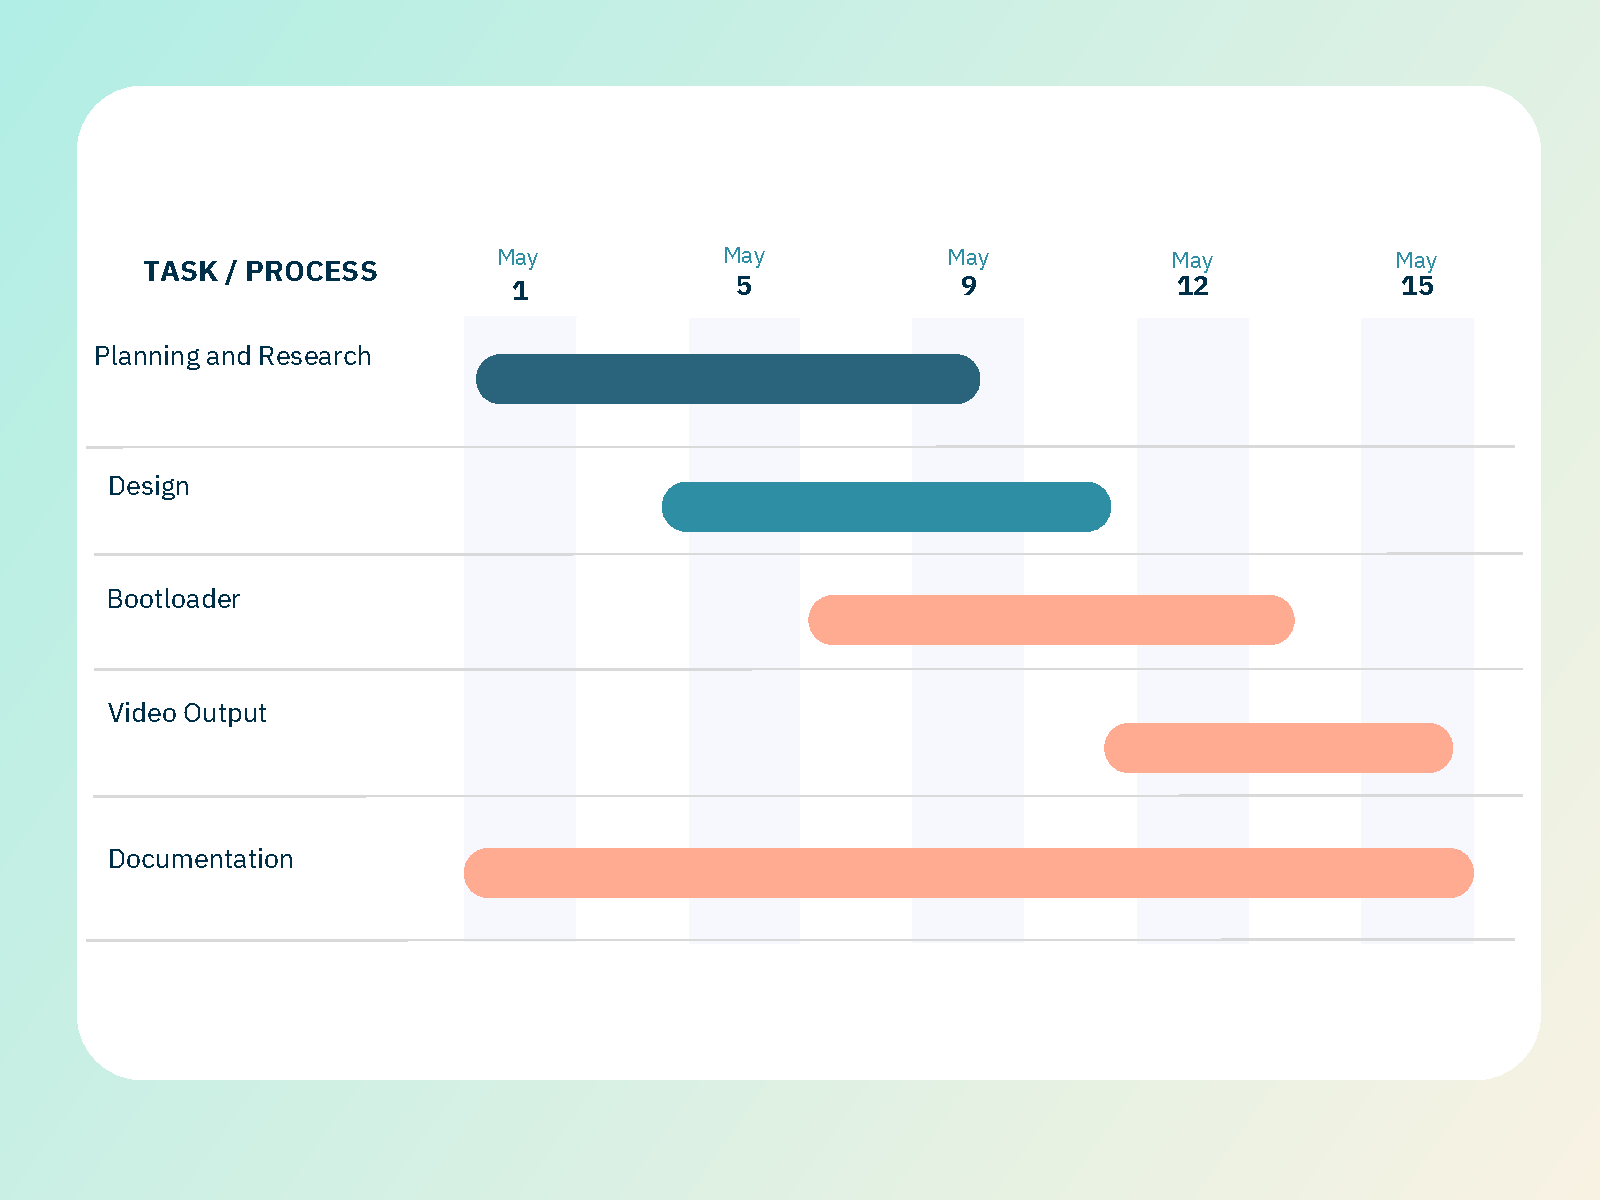
\includegraphics[width=0.8\textwidth]{figures/Increment1.pdf}
    \caption{Gantt Chart for Increment 1}
    \label{fig:Gantt Chart for Increment 1}
\end{figure}
\begin{figure}[H]
    \centering
    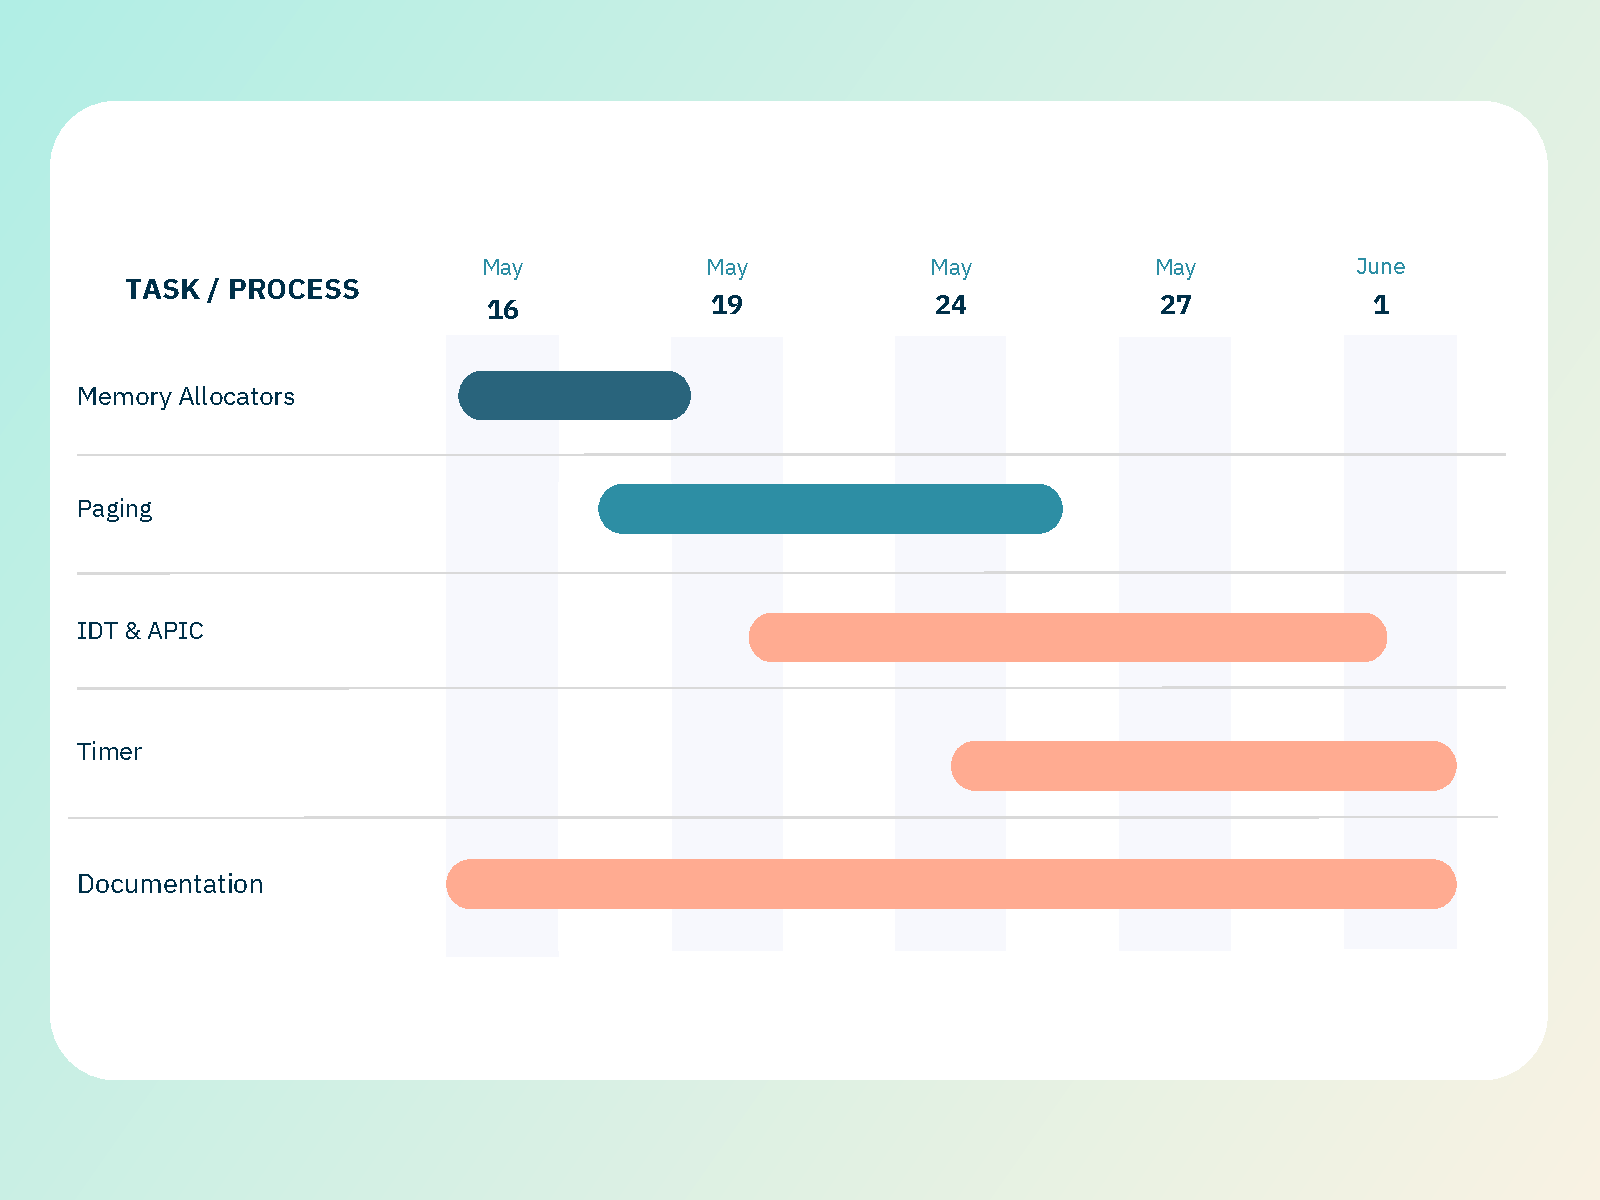
\includegraphics[width=0.8\textwidth]{figures/Increment2.pdf}
    \caption{Gantt Chart for Increment 2}
    \label{fig:Gantt Chart for Increment 2}
\end{figure}
\begin{figure}[H]
    \centering
    
\includegraphics[width=0.8\textwidth]{3.png}
    \caption{Gantt Chart for Increment 3}
    \label{fig:Gantt Chart for Increment 3}
\end{figure}
\begin{figure}[H]
    \centering
    
\includegraphics[width=0.8\textwidth]{4.png}
    \caption{Gantt Chart for Increment 4}
    \label{fig:Gantt Chart for Increment 4}
\end{figure}
\pagebreak

\section{Conclusion}

The KernelZ project successfully demonstrates the design and implementation of a 64-bit lightweight, memory-safe, monolithic operating system kernel using the Zig programming language. Developed from scratch, the kernel embodies modern systems programming principles while maintaining clarity and educational accessibility. Through a structured development lifecycle and modular architecture, KernelZ implements critical subsystems such as memory management, interrupt handling, scheduling, system calls, ELF binary execution, and a minimal virtual file system.

The use of Limine bootloader, QEMU emulation, and ACPI integration enabled robust testing and hardware abstraction, while Zig provided the fine-grained memory control essential for low-level kernel development. Each subsystem was rigorously validated via unit, integration, and fault testing to ensure reliability and correctness. By prioritizing modularity, transparency, and safety, KernelZ serves as both a functional operating system kernel and a valuable learning resource for students exploring system software development.
\pagebreak


\section{Future Enhancement}

Although KernelZ meets its initial objectives, several promising directions remain for future development and expansion:

\begin{itemize}
    \item \textbf{Symmetric Multi-Processing (SMP):} Support for Application Processor (AP) startup and CPU affinity will enable parallel execution and better utilization of multi-core architectures.
    
    \item \textbf{Persistent Storage Support:} Integrating drivers for storage devices (e.g., AHCI, NVMe) and adding support for disk-based filesystems (e.g., ext2, FAT32) will allow permanent data storage.

    \item \textbf{User Process Management:} Implementing process isolation, fork/exec semantics, and dynamic memory allocation in user space would enable multitasking with actual user applications.

    \item \textbf{Networking Stack:} Incorporating a basic TCP/IP stack and network device drivers (e.g., Intel E1000) will make the kernel capable of real-world communication and remote management.

    \item \textbf{Graphical User Interface (GUI):} Development of a simple window manager or graphical shell using framebuffer and input devices would enhance interactivity and user experience.
\end{itemize}

These enhancements would move KernelZ from an educational prototype to a more complete, general-purpose operating system suitable for advanced research, embedded environments, and custom computing platforms.

\pagebreak

\printbibliography
\pagebreak

\appendix
\addcontentsline{toc}{section}{Appendix}

\section{Screenshots}
This section contains screenshots captured during various stages of the boot
process to provide visual reference for the implementation. These images
demonstrate the successful execution and setup of the bootloader, serial console
output, and the system's initial booting screen.

Figure~\ref{fig:bootloader-menu-screenshot} shows the bootloader menu from
Limine, indicating a correctly configured booting environment.
Figure~\ref{fig:serial-logs-screenshot} displays the serial console logs, which
are useful for debugging and confirming the correct sequence of kernel
initialization steps. Finally, Figure~\ref{fig:booting-screen} presents the
booting screen output once the kernel takes over.

\begin{figure}[h]
    \centering
    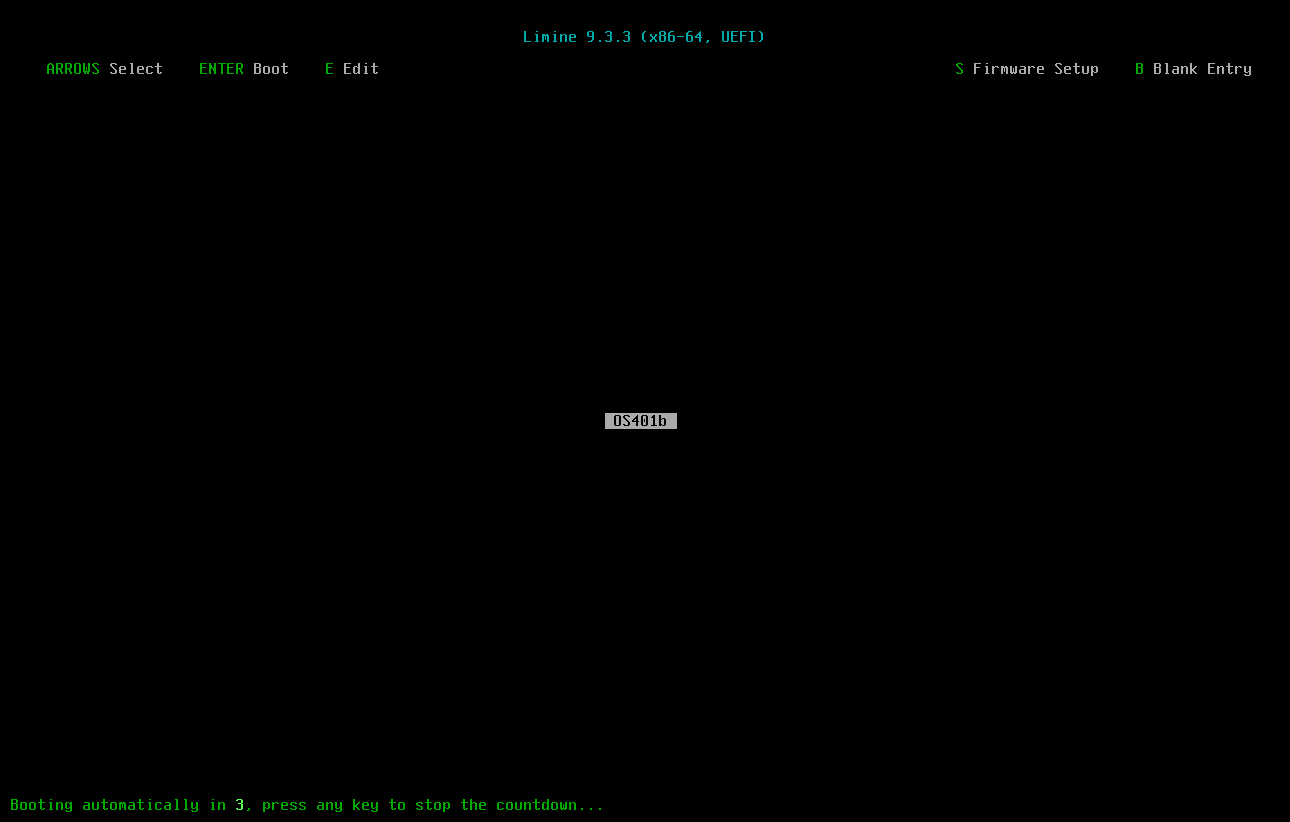
\includegraphics[width=1\linewidth]{screenshots/bootloader-menu.png}
    \caption{Bootloader Menu}
    \label{fig:bootloader-menu-screenshot}
\end{figure}

\begin{figure}
    \centering
    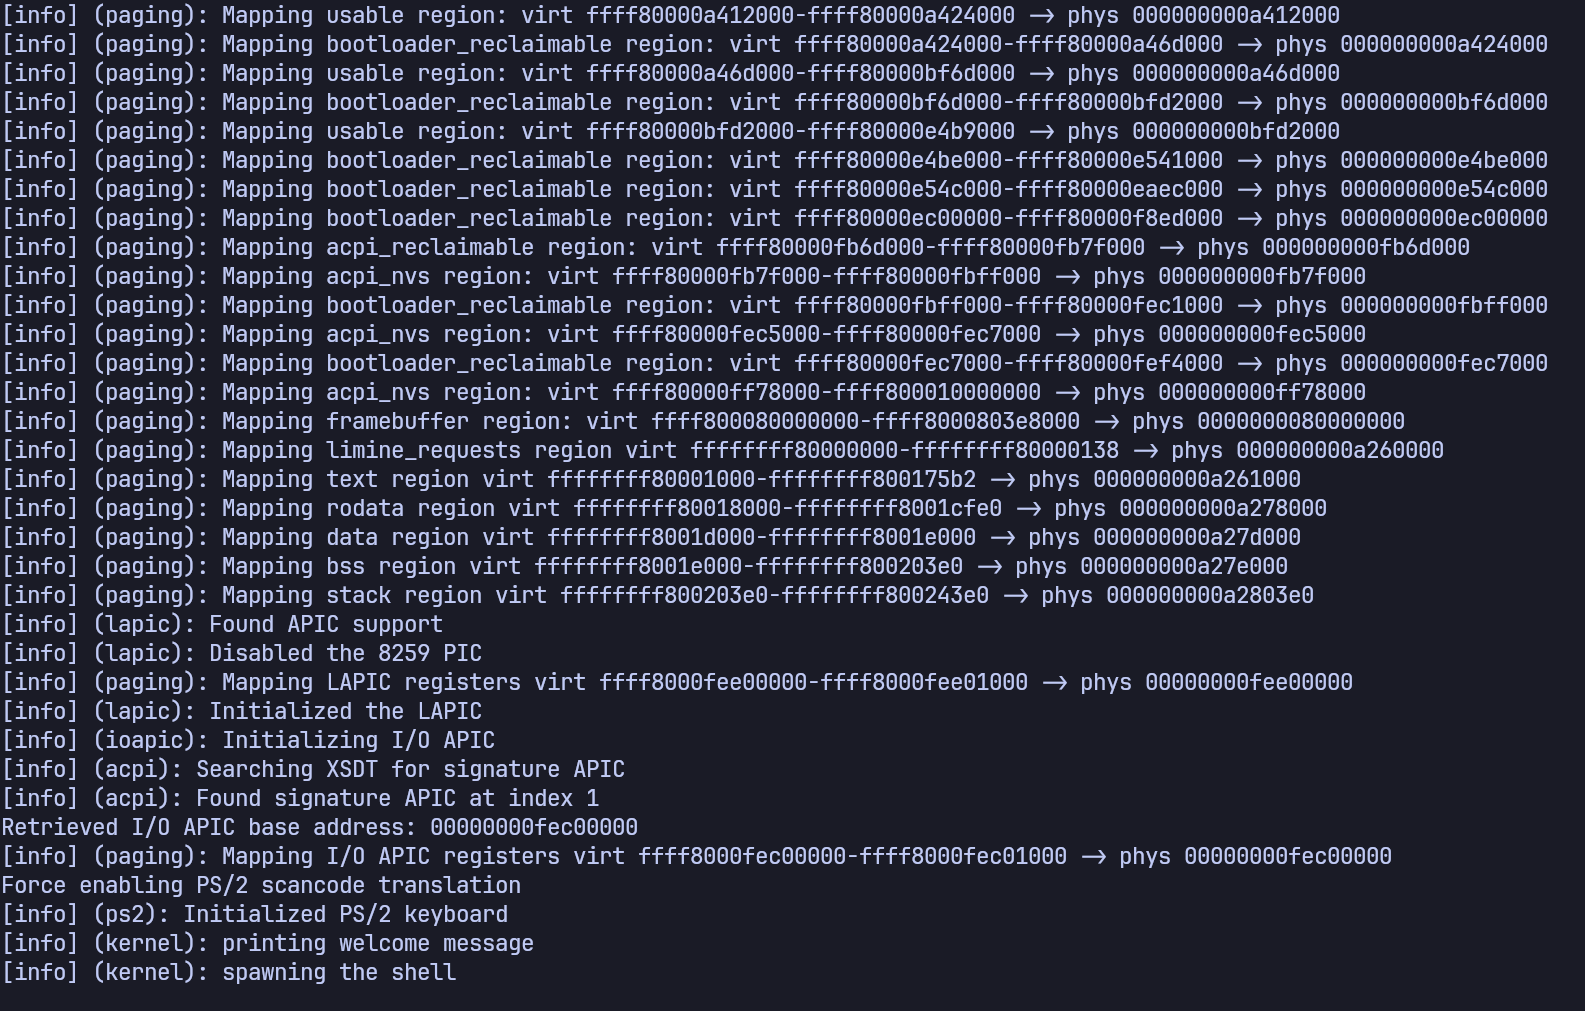
\includegraphics[width=1\linewidth]{screenshots/serial-console-logs.png}
    \caption{Serial console logs}
    \label{fig:serial-logs-screenshot}
\end{figure}

\begin{figure}
    \centering
    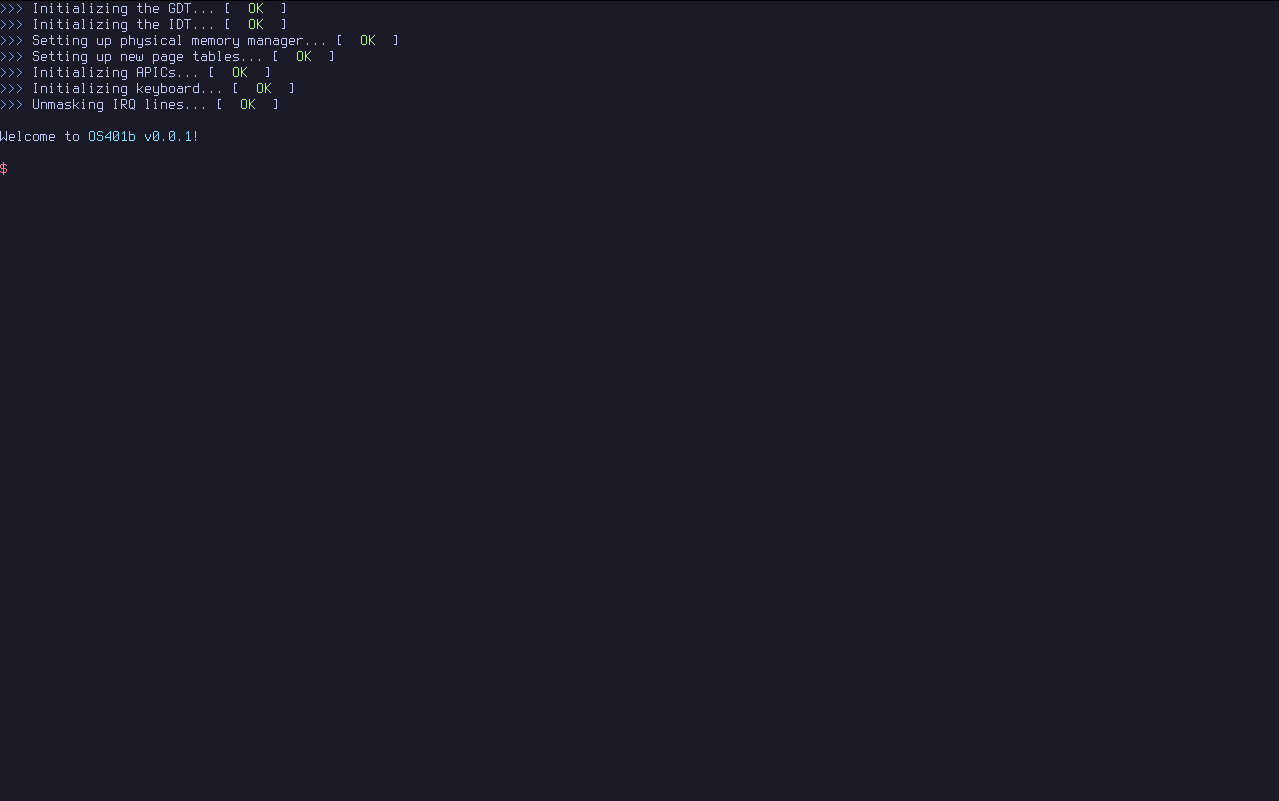
\includegraphics[width=1\linewidth]{screenshots/booting-screen.png}
    \caption{Booting Screen}
    \label{fig:booting-screen}
\end{figure}

\end{document}